\documentclass[11pt]{ociamthesis}  % default square logo 
%\documentclass[12pt,beltcrest]{ociamthesis} % use old belt crest logo
%\documentclass[12pt,shieldcrest]{ociamthesis} % use older shield crest logo
%load any additional packages

\usepackage{lmodern}% better font than default
\usepackage{tgcursor}% tt font with bold/italic styles
\usepackage{listings}
\usepackage{graphicx,wrapfig,lipsum}
\usepackage[colorlinks]{hyperref}
\usepackage{lscape}
\usepackage{amssymb}
\usepackage{multirow}
\usepackage{subfig}
\usepackage{makecell}
\usepackage[paper=portrait,pagesize]{typearea}
\usepackage{changepage}
\usepackage{enumitem}
\usepackage{multicol}

\usepackage{mathtools}
\usepackage[export]{adjustbox}
\usepackage[square,sort,comma,numbers]{natbib}
%input macros (i.e. write your own macros file called mymacros.tex 
%and uncomment the next line)
%\include{mymacros}

\title{Semantic Smart Contracts   %your thesis title,
      And Their Integration With Semantic Data Licensing} 
          %note \\[1ex] is a line break in the title

\author{Zahra Jafari \\
Supervisor: Priv.-Doz. Dr. Anna Fense} 

\college{Department of Computer Science \\
Semantic Technology Institute Innsbruck}

\degree{Master's Program\\ Computer Science}     %the degree
\degreedate{2023}         %the degree date


%end the preamble and start the document
\begin{document}

%this baselineskip gives sufficient line spacing for an examiner to easily
%markup the thesis with comments
\baselineskip=18pt plus1pt

%set the number of sectioning levels that get number and appear in the contents
\setcounter{secnumdepth}{3}
\setcounter{tocdepth}{3}


\maketitle                  % create a title page from the preamble info
\begin{dedication}
This page is intentionally left blank.\\
\end{dedication}        % include a dedication.tex file

 \centerline{This page is intentionally left blank.}

                  

   % include an acknowledgements.tex file
\begin{abstract}
\textit{Smart contracts as computer code which reside on blockchain, are receiving great attention in new business application 
because they allow parties to represent contract terms in program code and
thus eliminate the need for a trusted third party.
The creation process of writing valid, transparent contracts is difficult task.
Blockchain as distributed ledger technology is increasingly used as transnational data storage between parties and it gains good popularity among new industries in last few years. Blockchain implemented in different areas of applications such as social, healthcare, logistic and etc. It is also capable to execute smart contract and prevents data tampering by validating transaction through consensus protocol. 
Research on this topic is still on early stage in science. Since our goal is to analysis the way of integrating semantic web licensing using DALICC library and deploying smart contract, we divide this research 
into four sections: first we focused on how smart contract build up on blockchain. Second, we demonstrate how blockchain can integrate with semantic web technology. It is focused on some solutions for indexing and executing smart contract on Ethereum blockchain. And third section, It is focused on Data Licenses Clearance Center (DALICC) as a framework helps to detect license conflict and reduce the costs of rights clearance. And in the last section, we present project to present all these topics in the form of DApp.}

 



\end{abstract}          % include the abstract

\begin{romanpages}          % start roman page numbering
\tableofcontents            % generate and include a table of contents
\listoffigures              % generate and include a list of figures
\end{romanpages}            % end roman page numbering

%now include the files of latex for each of the chapters etc
\section{Introduction}

Etherem is one of the most popular blockchain platform which capable to generate decentralized application using smart contract. Ethereum is well-known for managing cryptocurrency using smart contract to automate this transaction.
It has been the best platform for developer coding smart contract in decentralized paradigm to generate decentralized application DApp.\\
Ethereum can be used in different scenarios, one strategy is to extract data from its blockchain network, linking  this data with the datasets of traditional web and query on them to generate new insight. \\
Another idea is, using semantic wen to standardize model and integrate data on web.  \textit{Tim Berners-Lee} described semantic web as model to extend web and allows to integrate machine with human. \\
Using semantic web enable access, integration and query on data sources, and create verity insight between different application domains. It uses ontology to allow query from the web using SPARQL and linking datasets. \\
Ontologies represent ethereum entities lick blocks, transaction message using RDF and Web Ontology Language(OWL). EthOn ontology formalize the concepts of ethereum blockchain on OWL, describing the ethereum objects as classes, data properties in ontology.\\
This thesis, we focused at two perposes: One ine to integrate semantic licenses from DALICC with smart contract. The other is to represent semantic model of deployed smart contracts. \\
This thesis present our efforts to build DApp to deploy smart contract in the presence of semantic licenses from DALICC, attaching licenses to contents, then applying semantic web techniques to link extracted date from ethereum transaction to semantic concepts adapted from Ethon ontology. \\
In the first chapter, we describe distributed ledger technology, blockchain, ethereum and some more details  to have better insight of used technology. In the next chapter, we represent some works around how semantic web can be applicable on blockcain. And on the last chapter, we present DApp to show smart contract integration with DALLICC semantic licences library and sementifying this deployment.




DALICC stands for Data Licenses Clearance Center is a framework that supports automated clearance of rights to help detecting license conflict and reduce the cost of high transaction related to manually clearance of licensing contents.
DALICC will develop and  integrate different functionalities that allows the automated clearance of rights issues.\\
In this thesis, deals with two things: One is the problem of linking license to contents for this purpose, we use Therefore, this work aims to find an appropriate and
generic method to attach semantic licenses to data and content. To achieve this, an
approach with a blockchain was chosen to design the entire system in a decentralized
and therefore trustworthy manner. Specifically, the Ethereum Platform was chosen,
because it is one of the most popular platforms for decentralized applications in the\\
Smart contract is computer program that expressed the content of agreements and preform transaction on blockchain when specific conditions are met. Smart contract preform verified transaction on blockhain without third party or any supervisors, thus ensuring us to transparent, valid and secure transaction.
AS Blockchain as distributed ledger become much popular and widely used in many field, the need of making query of such data becomes more important.
As blockain is distributed ledger which store data and transactions, querying them becomes challenges task. This due to the fact that blockchian can allow transaction and payment without needing intermediary.
Moreover there is need to integrate blockchin with semantic web service, thus making use of some linked data tools to index blocks and transaction according to Ethereum ontology.  \\

\chapter{Smart Contract and Distributed Ledger Technology}
With the advances in technologies, transferring money is done over networks, and we just need to update related database entries that are controlled by central authorities like banks. These all processes need to third party to make appropriate transactions between unknown parties. \\
There are many problems with having third parties such as controlling the whole transaction by single authority, invalidating any transaction to serves their purpose . All these issues can be resolved using the novel idea of a distributed ledger. In this new technology, the third parties is eliminated, and all transactions will be done over the public network between parties within minutes. \\
With the presence of new technology, no one can manipulate transactions stored in a ledger or trace the involved parties in these transactions \cite {Masood}. 
\section{Ledger} 
A ledger is a book or computer that records transactions associated with a financial system. There are two different ledgers as below: \\
\textbf{Centralized Ledger} contains all recording transactions related to company assets, costs, libraries, etc. \\
\textbf{Decentralized Ledger} is a database that shares data across the network. It allows transactions to be executed in public. Any participant of each node can have an identical copy of the ledger, which is already shared on the network.\\
If any change or update occurs on the ledger, each node constructs a new transition and votes by the consensus algorithm to choose the correct copy of the ledger. Once the consensus has been done, other nodes will be synchronized with the latest version of the ledger \cite{Markos}.

\section{Distributed Vs. Decentralized } 
The difference between decentralized and distributed is made by Baran (1964) \cite{Baran}. Decentralized means that there is no single authority to make a decision. Each participant can make a decision individually, and the system gathers all responses as resulting behavior. However, there is no single authority in the distributed system too, but the process is spread across all participants and decisions will be centralized. The main difference between distributed and decentralized is that a decentralized database is a collection of inter-connected databases that work independently in different locations. Ozsu et al. \cite{Ozsu} define a distributed database as a "collection of multiple, logically interrelated databases distributed over a computer network and distributed database makes a transparent distribution to all users" \cite{Ozsu}. Based on this definition, blockchain technology covers both types, as it appears as a single system to its users and performs a task across a network. Thus, blockchain is a form of a distributed database system \cite{Markos}.


\section{Distributed Ledger Technology (DLT)} 
DLT refers to a database that provides identical copies of shared data among participants which would be updated using a complex consensus mechanism between participants. It is used to reduce the costs and increase transparently, traceability, and speed of the process.\\
This technology involves many challenges, and some of them have not been resolved so far. The most common challenges of DLT concern scalability, inseparability, and data privacy \cite{Jose}. \\
\\
\textbf{How does DLT work?}\\
\\
DLT is the result of combining main three technologies:\\
\hspace{1cm}\textit{-  P2P}: all participants (nodes) act simultaneously as client and server, consuming and contributing resources.\\
\hspace{1cm}\textit{- Cryptography} is used to authenticate the identity of the participant and the information between the two parties. Using encryption helps prevent third parties from accessing information. \\
\hspace{1cm}\textit{- Consensus algorithm} allows network participants to come into agreement to add a new node (block) to the ledger \cite{Jose}.\\
\section{Blockchain} According to what World Bank Group \cite{Natarajan} referred, blockchain is the most popular distributed ledger that stores and publishes data in packages called "blocks". Each block contains information such as nonce, timestamp, block hash, and a hash pointer to the previous block in its header. Therefore, all these blocks are connected in a digital chain \cite{Natarajan}. \\
Luke et al. \cite{Luke} refer to blockchain as a list of blocks that are linked to each other and secured cryptography. The participants on networks have an identical copy of these records stored locally on the computers of all participants. Blockchain starts processing, when the user request transaction whether is a transaction, contract, or other information. The transaction is broadcast on P2P network of nodes. Following that, the verification process takes place where all of the nodes in the P2P network verify the transactions via the hashes which are generated by some algorithm. Once verification is completed, transaction detail will be stored in a block. Finally, a new block is added to a chain in a way that is permanent and unchangeable \cite{Luke}. The initial block in the blockchain known as \textit{Genesis} block, the other nodes will be added to the chain after the process of consensus between nodes. The consensus mechanism allows the blockchain to grow without fear of manipulating the information of blocks. Since the blocks contain transactions, the consensus process takes place in a predefined time interval. This interval is the duration of when the initiation of the transaction took place and the addition of the transaction into a blockchain. This confirmation time is varied based on block size, transaction, and consensus algorithm. There are different methods for consensus mechanism listed: 
\begin{itemize}
    \item Proof of Work (PoW): 
    It is a mechanism that ensures consensus is done without any central control. By the usage of this mechanism miners compete to complete their transaction first into blockchain and get rewards (e.g: Bitcoin, Ether).\\
    Miners (actors who participate in cryptocurrency transactions) connect to blockchain and accomplish tasks validating transactions to add new blocks by solving a cryptographic puzzle and anybody who completes their task sooner can add their block first in blockchain \cite{Pablo}.
    \item Proof of Stake (PoS): 
    It is an alternative to proof-of-work that fewer CPU computations for mining. In proof of stake, the chance of mining the next block depends on node balance. 
    In private networks, however, where the participants know each other, consensus mechanisms such as proof of work are not required. This particularly removes the need for mining and gives us more variety of consensus protocols for picking from \cite{Christidis}.
    \item Proof of Authority (PoA): It confirms accounts and allows them to add a transaction in blocks. Since this approach is much more centralized and transaction speed is faster, is prone to be attacked more than the other methods \cite{Luke}.
    \item Practical Byzantine Fault Tolerance (PBFT): Blockchain tries to solve the problem called 'Byzantine Generals' which refers to some members on the network who send incoherent or fake information related to the transaction to others. Since there is no authority on blockchain to correct them, leads to the unreliability of blockchain. PBFT algorithm tries to achieve a consensus to solve this issue in a way that uses the concept of primary and secondary vote. Secondary vote automatically evaluate the decisions made by primary vote and can collectively change to a new primary, if primary vote is compromised \cite{Luke}.
\end{itemize}
Blockchain is associated with cryptocurrencies like Ethereum, bitcoin, lite coin, etc. Gupta (2017) \cite{Gupta} identified five core attributes which blockchain builds trust through them:
\begin{itemize}
    \item Distributed ledger: The data is not controlled by any single authority. It is shared, and updated across the network and the new changes will be replicated to all participants.
    \item Orchestrated and flexible: Since smart contracts can be executed on the blockchain. The blockchain can be evolved to support business processes and activities.
    \item Transparent and auditable: There is no need for a third party or another authority, as all participants have access to the same ledger, verify transactions, and identify the owner. 
    \item Secure, private, and indelible:
    Blockchain provides these features using some capabilities such as permissions and cryptography which ensures that  
    unauthorized users do not have any access to the network. It means that participants are really who they claim.
    \item Consensus: All nodes on the network should agree to validate transition and blockchain perform this process by consensus algorithm \cite{Gupta}.
\end{itemize}
\\
\textbf{Type of Blockchain} \\
\\
According to Aithal et al. \cite{Aithal} blockchain is used to transfer and exchange information through the secure network. Primarily, there were two types of blockchain technology: public and private networks. Based on some other analysis, blockchain can also be noted as consortium blockchain technology and hybrid blockchain technology \cite{Aithal}. \\
That should be noted that all kinds of blockchains consist of nodes and works on P2P peer-to-peer network. Aithal et al. \cite{Aithal} classified blockchain into three types as bellow: public blockchain, private blockchain, and consortium blockchain. Besides this, there is another type of blockchain, known as the hybrid blockchain.
\begin{itemize}
    \item \textbf{Public Blockchain} is the main type of blockchain that, is decentralized and open naturaly. In this system, anyone is allowed to join to network and create consensuses. In a public blockchain, any miner (participant) can create consensus mechanisms such as proof of work, and proof of stake to validate the transaction with a low rate of validity \cite{Kalra}.
    \item \textbf{Private Blockchain} is not open and restricted in a way that the only restricted participant has the right to validate the transaction. Therefore, it provides better privacy, improves scalability, and mitigates security issues. This blockchain does not have mining computation to reach the consensus because all participants are known in this network \cite{Kalra}. 
    \item \textbf{Consortium Blockchain} is semi-decentralized blockchain and is used to do activities for a single organization like bank, etc. The difference between private blockchain with this type is that Consortium Blockchain is controlled by a group rather than a single authority \cite{Aithal}.
    \item \textbf{Hybrid Blockchain} is a combination of public and private blockchains. Thus, it makes the benefit of privacy in private blockchain combined with the security and transparency of the public blockchain. In this type of blockchain, the user can control who gets access to which data on the blockchain. A transaction can be verified in a private network, and the user can release it to the public blockchain. By doing so, only selected parts of the records can be accessible in public and the rest could still maintain confidential in a private network \cite{Aithal}. 
\end{itemize}

 \section{Ethereum}
Ethereum is the most active public blockchain in the world at present. It is another cryptocurrency similar to Bitcoin that is built on top of the blockchain. The participant publishes the transactions on the network, which are then stored in blocks and added to the blockchain using a consensus mechanism. The term state in Ethereum refers to the state of different accounts pupulating on the blockchain. An account in Ethereum can either be an external account related to the user or a contract account that obtains constant storage in the blockchain. The virtual currency in this system is \textit{Ether}. The transaction can change the state of the system by creating a new contract or invoking an existing contract \cite{Ilya}.

\section{How does Ethereum works?}
In this subsection, we will focus on the Ethereum workflow at a technical level.
\subsection{Blockchain}
The blockchain contains some information that we have used in our project. Therefore we focus on it more, as below:
\begin{center}
	\begin{figure}[htb!]
		
		\begin{minipage}{0.5\linewidth}
			\centering
			\includegraphics[width=1.95\textwidth]{images/chap01_Blockchain.png}
		\end{minipage}
		\caption[Block contents]{Block contents \footnote{https://archive.researchworld.com/three-ways-that-blockchain-can-improve-the-quality-of-market-research/}}
		
	\end{figure}
	
\end{center}
\begin{itemize}
    \item \textbf{Block} as a data structure within the blockchain contains different functions which include transaction hashes and some other additional information for blockchain technology. Gavin Wood et al. \cite{Gavin} described some relevant information below and we used this information in our project: \\
    \begin{itemize}
        \item \textit{parentHash} is the hash of the parent block’s header.
        \item \textit{sateRoot} is the hash of the root node of the state, after execution of all transactions are applied.
        \item \textit{transactionRoot} is the hash of the root node of data populated with a transaction in the transactions list inside the block.
        \item \textit{receiptRoot}is the hash of the root node of the data populated with the receipts of transactions in the block.
        \item \textit{logsBloom} composed of log information.
        \item \textit{difficulty} represents the difficulty level of the block.
        \item \textit{number} is the number of ancestor blocks.
        \item \textit{gasLimit} represents the current limit of gas in the block.
        \item \textit{gasUsed} is the amount of gas used for the transaction in the block.
        \item \textit{timestamp} is time of reasonable output.
        \item \textit{extraData} is a byte array containing relevant information in the block.
        \item \textit{nonce} is number of several computations that have been done in the block.
    \end{itemize}
  \item \textbf{Mining} is a process of computation on the blockchain to verify and add a block. The miner adds a new block, and others check the validity of the new block. Any participant can take part in the mining pool, but the chance of finding a valid block depends on the power of the computer to perform calculations. Sometimes a miner will find an uncle block. 'An uncle block is a block that is initially valid but is surpassed by another faster block'. An Uncle block is rewarded with $\frac{7}{8}$ of full block value, and a hash will be added to a valid block. A maximum of two uncle blocks can be added to a valid block, and the miner of the valid block also receives $\frac{1}{32}$ extra Ether for each uncle block \cite{Egbertsen}.
    \item \textbf{Mining pool} is a way that miners gather together, start mining, solve blocks, and win rewards, and then the reward will be split among the involved miners \cite{Egbertsen}.
\end{itemize}
\subsection{Ether}
It is the form of payment and fuel for Ethereum. The base for mining (finding the solution and adding blocks) successfully is five ethers. If the miner finds a solution but not fast enough, it becomes less ether, like 4.375 ether, and will be an uncle block. Each block can contain just two uncle blocks and receive $\frac{1}{32}$ per uncle block. If another miner also finds a solution. This block cannot be added to the blockchain, and the miner just receives 2-3 ether \cite{Egbertsen}.
\subsection{Account}
There are two types of accounts in Ethereum:\\
- \textit{Normal account} is controlled by the private key. The owner of this account can send ether or a message.\\
- \textit{Contract} account is controlled by code. It can only fire a transaction in response to other transactions \cite{Egbertsen}. An account encompasses four fields:\\
 \begin{itemize}
     \item \textit{nonce} is the number of transactions sent from this address \cite{Gavin}.
     \item \textit{balance} is the number of Wei owned by this address \cite{Gavin}.
     \item \textit{storageRoot} is the hash of the root node of the Merkle Patrica tree, which encodes the content of an account. It should also be noted that the Merkle tree is used for data representation in the block header \cite{Gavin}.
     \item \textit{codeHash}
     is the hash associated with this account that would be executed when this account address receives a message call and would not be changeable anymore. All information about this account is stored in the database under the corresponding hash code for later retrieval \cite{Gavin}. \\
    
\end{itemize}
\textbf{Hash function}
is the process of SHA3 standardization at National Institute of Standards and Technology (NIST) was completed in August 2015.
This standard specifies the SHA3 (Secure Hash Algorithm-3) family of functions for binary data. Each hash function is based on \textit{Kacak} algorithm, known as NIST, the winner of the SHA3 cryptographic hash algorithm competition. The SHA3 family includes four functions with different lengths of 224, 256, 384, and 512 bits.
In the hash function, input is called as \textit{message} and output is called as \textit{has value} where the length of the message can vary but the length of the hash value is always fixed \cite{Dworkin}.\\


\begin{center}
	\begin{figure}[htb!]
		
		\begin{minipage}{0.2\linewidth}
			\centering
			\includegraphics[width=4.5\textwidth]{images/chap01_hash_function.png}
		\end{minipage}
		\caption[Image of hash function]{Image of hash function \cite{Dworkin}}
		
	\end{figure}
	
\end{center}
\textbf{Gas} is fuel on the Ethereum platform that is paid before executing a transaction. In a case that the transaction is rolled back, the consumed gas will not be returned \cite{Egbertsen}.\\
\begin{itemize}
    \item \textbf{Transaction}
     Gavin Wood et al. \cite{Gavin} described a transaction as a cryptography-signed instruction that is executed by an external actor, which can be a human or another contract. The transaction describes these fields:
     \begin{itemize}
         \item \textit{nonce} is the number of transactions sent by the sender.
         \item \textit{gasPrice} is the number of wei to be paid per unit of gas.
         \item \textit{gasLimit} is the amount of gas that can be used for transactions.
         \item \textit{to} is the address to which that contract sends a transaction.
         \item \textit{value} is the number of wei that is transferred in the transaction.
     \end{itemize}
        \item \textbf{Message} is fired by contract and contains all attributes the same as a transaction, but $gasPrice$ \cite{Egbertsen}.
\end{itemize}
\subsection{Contract} 
It is an account on the Ethereum blockchain that has its own code and is controlled by code. The code inside the contract is triggered whenever it receives a message, allowing it to read and write contract storage or send a message. \\
A contract in Ethereum is an autonomous agent that performs some operations that are programmed to fulfill the user's goals, meaning that the contract is an autonomous agent that is executed when it receives a message or transaction, having control over its balance and the key/value store as constant variables.
The keys and values stored in the contract are long-lasting and get used whenever the contract starts running \cite{Egbertsen}.

\subsection{Smart Contract}
The term smart contract was coined in 1994 by Nick Szabo \cite{Szabo} who released that DLT can also be used for smart contracts.
According to Nick Szabo \textit{"Smart contract is a computerized transaction protocol that executes the terms of a contract"}\footnote{https://www.fon.hum.uva.nl/rob/Courses/InformationInSpeech/CDROM/Literature/LOTwinterschool2006/szabo.best.vwh.net/smart.contracts.html}. He visualized an away to write agreement that enforces the conditions between parties involved in a transaction automatically and more efficiently.
Smart contracts are run by each node as part of the block creation process. Block creation occurs when transactions take place in the block.
An important part of a smart contract is that each contract has its own address. Since the contract code is carried to the transaction, a node can create the specific transaction, assigning an address to the contract, and this transaction is capable of running contract code at the time of creation.\\
After that, the contract will be part of the block, and the address will never change. Whenever the node wants to call a method inside the contract, it should send a message to the address of the contract that has the method and input data.
The contract will run as part of the creation of a new block and then return value or store data on the blockchain \cite{Payrott}.\\
\\
\textbf{Solidity} is a high-level, truing complete language with a Java script similar syntax. The contract is similar to classes in an object-oriented language, which contain fields for persistent storage of contracts and methods to be invoked by internal and external transactions. For interacting with another contract, we either need to create a new instance of this contract or make a transaction to a known contract address.\\
In principle, Solidity provides some basics to access blocks and transaction details, like: \textit{msg:sender} for accessing the address of an account or \textit{msg:value} to access the amount of \textit{wei} transferred by the transaction. It also uses some functions to transfer money to another contract, such as \textit{call} and \textit{send}. These functions get used to transfer value and translate into an internal call to a transaction, which causes the contract to also execute code or may fail to execute due to insufficient gas \cite{Ilya}.
\chapter{Block chain as infrastructure of semantic web}[paper6]



\section{Distributed ledgers and indexing}[p1431]
Distributed ledger based on blockchain do not have central control. Blockchains are organized into multiple blocks that initial block created manually and the other blocks are added by some consensus process between nodes.
Ethereum smart contract provides possibility of to control automatically what happen with cryptocurrency on the blockchain without involving the untrusted external sources. Ethereum smart  contracts has account which can normally store, update or making function with the input and output.
The concept\textit{accounts} are widely used in this study refer to agent such human and the concept \textit{balance} refers to cryptocurenccy in blockchains. \\ 
As already said, smart contracts are time-ordered where data are stored into blocks. therefore it requires the data to index. Indexing the smart contract, gives us capability to access the data, search, analysis services on the distributed ledger and expose them to outside the worlds for more of interactions.
There are different levels of indexing smart contracts: Basic level is the fundamental level for next step.It index basic entities such as account, blocks related to distributed level and data can be stored or retrieved here. In functional level, smart contracts contains alot of functional interfaces that depict the other functionality of platforms such as Ethereum. [p1431]
 There are not such comprehensive vocabularies to describe such concepts but some vocabularies are purposed in this case such as: 
\\
\textbf{FlexLedger}   
\textbf{BLONDiE and EthOn}  are formalisations of blockchain concepts
as ontologies, generic across Bitcoin and Ethereum blockchains and specifc to
Ethereum, respectively. It discuss initial approaches to Linked Data
indexing of blockchains, and the certication of Linked Data temporal streams
on blockchains, but both are very preliminary.[53]
  
 \section{Vocabularies}[p1431]
 \subsection{Why do we use ontology for Blockchain?}
 GEnerally, Blockchain is the destrubuted database that replicated over all nodes as s cloud computing arcitecture. These databases are distributed across noumerous organizations. That's why standard interpretation is needed that the data would be understandable by organizations. Interpretations are applicable via formal specification that enable verification and inference within software and applications executed on network. \\
 This is where ontology to play to ensure common interpretation of data of shared database among different intersperses. Blockchain modeling is the one form of modeling among enterprises.
 blockchain modeling used different type of ontology: informal ontology, semi ontology to facilitate search and enhance better understanding of business process for developing and applying on blockchain. Blockchain modeling based on formal ontology help the formal specification to verify the operation of blockchain. On the other word, blockchain modeling based on formal ontology can help the development of smart contract to execute on blockchain.\\
 Also, we can use ontology tocapture data within blockchain: From one hand, It facilitates the better understanding of blockchain concepts for human.On the other hand, enables interlinking with other link data to convey deductions and formal reasoning.[2]\\
 Vocabulary used within ontology increase the transparency of transaction in a way that by describing transaction in the context of linked data comfort the graphical represantation of location of such transaction. Thus , it increases also the capability of analysis by users.
   
 \begin{center}
 
 	
 	\begin{figure}[htb!]
 		
 		\begin{minipage}{0.55\linewidth}
 			\centering
 			\includegraphics[width=1.65\textwidth]{images/chap02_diagram_ontology.png}
 		\end{minipage}
 		\caption[Illustration of Ontology diagram]{Illustration of Ontology diagram(2)}
 		
 		
 	\end{figure}
 	
 \end{center}
 
\subsection{Linked Data}
TODO
when information can represenr in linked data, querying about realted information can be easily discovered in linked data. It is based on 4 rules:

	\textbf{URIs}(Uniform Resource identifier) as names.\\ 
	\textbf{HTTP} to search for names.\\
	\textbf{(SPARQL, RDF)}  when a user search for something, provides related information.\\
	\textbf{Link} to other URLs to provide more information.\\


\subsection{Resource Discription Framework}
It is w3c specification that model information.
TODO
\subsection{SPARQL}
TODO
\subsection{Ontology and OWL}
TODO
Ontology Wen Language is made to represent knowledge bout things and the relations among them. OWL is computational logic-based language ,means the language modeled in OWL can operated in computer program like negation, intersection and so on. TODO

 \subsection{Vocabulary in Distributed Ledger}
 In ord is replecated over allnr to generate link data, it requires to use a standard ontology or vocabulary to explain the blockchain concepts. Interfaces between distributed ledgers and the Semantic Web are still on early stage in this. there are some systems that have such voicabularie includes: Flex Ledger, EthOn, BLONDiE[p1431].\\
 
 \textit{FlexLedger}: describes HTTP interfaces to blockchains, with a standard vocabulary and responses of these interfaces[p1431]. FLexLedger is a protocol for decentrelized ledger and interfaces which represent ledger creation, querying and data model using JSON-LD. However, Flex Ledger does not have explicit vocabulary about ontology nor  having concrete ontology for itself. 
 \\TODO It is also worth mentioning that the Flex Ledgermeta and the content data are stored together in the same graphwhereas the GraphChain blocks’ content is store outside the blockin a separate graph. For all the reasons stated above, GraphChaincannot be considered as an implementation of Flex Ledger.[p1171]\\
 \\
 \\
 \\
 \\
 
 \textit{EthOn} is an OWl ontology that describes blockchain concepts such as \textit{"blocks, accounts, message"}and relations such \textit{"has parent block"}.[40] TODO
 \begin{center}
 	\begin{figure}[htb!]
 		
 		\begin{minipage}{0.55\linewidth}
 			\centering
 			\includegraphics[width=1.85\textwidth]{images/chap01_EthOn.png}
 		\end{minipage}
 		\caption[EthOn classes]{EthOn Classes(negotitaion)}
 	
 	\end{figure}

 	\begin{figure}[htb!]
 		
 		\begin{minipage}{0.55\linewidth}
 			\centering
 			\includegraphics[width=1.65\textwidth]{images/chap02_EthOn_Properties.png}
 		\end{minipage}
 		\caption[EthOn Properties]{EthOn classes(negotition)}
 		
 		
 	\end{figure}
 	
 \end{center}

\textit{Blockchain Ontology with Dynamic Extensibility(BLONDiE)}
	
BLONDiE is another OWL ontology for describing the
Blockchain structure like EthOn. But is is more generic then EthOn. For example EthOn and BLONDiE bothe defined some terms such 'account', 'block', 'transaction' and some attributes such as 'transaction payload' or 'miner adddress'. BLONDiE defines some other concept for different Blockchain such as 'BitcoinBlockHeader' and 'EthereumBlockHeader' as sub classes of 'BlockHeader'. At the moment, BLONDiE supports two crypocurrencies like bitcoin and Ethereum where all link and relation between objects and attribute represent in RDF(Resource Description Framework).[p1431]
\begin{center}
	\begin{figure}[htb!]
		
		\begin{minipage}{0.55\linewidth}
			\centering
			\includegraphics[width=1.95\textwidth]{images/chap02_BLONDiE.png}
		\end{minipage}
		\caption[BLONDiE]{BLONDiE usage example[45]}
		
		
	\end{figure}
	
\end{center}

\subsection{Linking Blockchain in BLONDiE[45]}TODO
On a general point of view, the Web is a huge global graph
of connected hypertext documents by hyperlinks. On a similar
way, there are some projects working in the idea of connecting
different Blockchains. Where the main goal is to create “the
Internet of Blockchains”. Since payments are different from
plane information, it can be copied and replicated, but money
must not be.
The interledger protocol (ILP)8 is for payments across
payment systems. ILP models the world of finance as a giant
global graph of ledgers connected by liquidity. The systems
providing this liquidity are called connectors and a key feature
of ILP is that these connectors do not need to be trusted,
meaning anyone can create one [21].
Currently, centralized exchange platforms are used to exchange
one Blockchain-based currency for another. Cosmos9
is a network of Blockchains, organized on hubs and zones.
Zones plugged into a central hub and each zone maintain
its each governance. Allowing the decentralized exchange of
tokens from one Blockchain to another.
Polkadot10 is a new network that aims to provide interoperability
between private and public Blockchains. Allowing
extensibility and scalability. It defines a heterogeneous
multi-chain, provided to an absolute minimum of security
and transport. Scalability is addressed through a divide-andconquer
approach. The heterogeneous nature of this architecture
enables many highly divergent types of consensus systems
interoperating in a trustless, fully decentralized “federation”,
enabling open and closed networks to have trust-free access
to each other [23].
Two more similar projects are Blocknet11 and Supernet12.
All these projects show evident need of semantic empowerment.
The same need that the web still has to really jump from
an only “Syntactic Web” (Web of documents) to a “Semantic
Web” (Web of data). While how and where to locate and
enable semantic data is not completely clear, it is obvious
that Semantic Web fits as a prominent set of technologies to
be used here. In Figure 4, we present datasets that have been
published in Linked Data format by contributors to the Linking
Open Data community project and other individuals and
organizations. In a similar way, Blockchains-based systems
and its corresponding datasets can be published and linked.

\begin{center}
	\begin{figure}[htb!]
		
		\begin{minipage}{0.55\linewidth}
			\centering
			\includegraphics[width=1.95\textwidth]{images/chap02_LinkData.png}
		\end{minipage}
		\caption[Linked data diagram]{Linked data Diagram[45]}
		
		
	\end{figure}
	
\end{center}

\subsection{Ontology-based smart contract in BLONDiE[45]}
Data models are used on Ontology-Based Object-Oriented
Enterprise Modelling [24]. In a similar manner, Kim and
Laskowski [25] propose that ontologies can contribute to
Blockchain design. Their approach can aid in the development
of Smart Contracts that execute on the Blockchain.
They come up with a proof-of-concept using Ethereum
and TOVE Traceability Ontology. This interesting idea can
be replicated for other ontologies too. Better data standards,
business practices and processes for developing and operating
Blockchain are achieved. It also aids in the formal specification
for automated inference and verification in the operation of a
Blockchain.[45] TODO

\subsection{Storage and RDF}
The main goal of data over web is to make data machine readable format on web. It causes to interpret data in suitable formats to be useful in a way that be human readable too. \\
JSON-RPC is remote procedure call protocol in JSON. his protocol allows to send data to server without needing to response. 
Ethereum blockchian which has properties such as pay 
fee with Gas, there are different was of storing data in RDF triple
Most wallet in Ethereum in in JSON format that is seasily convertble to RDF and fornt-end is made up with HTML  technology that we can use it to embed data on website interface as Micro data, JSON-LD. The main focus of research is the storage of data on blockahain itself.There exist limitation of storage in Ethereum blockchain and to fees. that's why, it is suitable to use compact RDF serialization.[45] There are some methods to store data on Ethereum  blockchain that are summarized in table bellow:
\begin{center}
	\begin{figure}[htb!]
		
		\begin{minipage}{0.55\linewidth}
			\centering
			\includegraphics[width=1.95\textwidth]{images/chap02_Eth_str.png}
		\end{minipage}
		\caption[Ethreuem structure]{Ethereum structure}
		
	\end{figure}
	
\end{center}
\begin{center}
	\begin{figure}[htb!]
		
		\begin{minipage}{0.55\linewidth}
			\centering
			\includegraphics[width=1.95\textwidth]{images/chap02_Eth_Table.png}
		\end{minipage}
		\caption[Storage of RDF data on Ethreuem summery]{Storage of RDF data on Ethreuem summery}
		
	\end{figure}
	
\end{center}



\subsection{Semantic Blockchain}
	
By increasing of the usage of blockchain technology recently, the need for semantic reasoning on distributed ledger is on crease as well. The blockchain is the best platform to utilize semantic web principle inthis technology and add new trusted property to dataset. that makes new dataset so thruthworthy. 
Using semantic web technology on blockchain in novel idea and the way of how apply this technology in blockchain and smart contract is also as controversial issue.\\
There are some \textbf{definition of semantic blockchain:}\\ 
\textit{Semantic blockchain is the representation of stored data on distributed ledger using linked data. }\\
\textit{Semtcic blockchian is the applying semantic web standard on blokchain that these standards is based on RDF.}

\subsection{semantify Blockchain process}
Semantic blockchain or semantic distributed ledger has effect on industrial world and subsequently , the result lead to start developing new application and framework to combine two worlds:
thee are some way to semantify blockchain:
\textbf{-}Mapping the basic blockchain to RDF making usege of vocalbularie, ontology and so on.
\textbf{-} Storage of data in blockchain is expensive, The only wey is to store the hashing point to data set in blockchain and then share RDF on blockchain.
\textbf{-} Create semantic blockchain that internal data exchange protocol is based on RDF.

TODO
SemBlocRouter [45]
\subsection{Semantic Ontology Mapping}[p1341]
To generate RDF, ot is need to ap the basic blockchain  etities to relevant semantic web terms, concepts and ontology. In order ot make query more efficent BLONDiE used some ways such as:\\  
Firstly, records realting to block and transactions both, have been completed with attribute for hashing to provide direct mapping between contents of index and address of entities on blockchain, Secondly, transaction with link to blocks or smart contract and input to smart contract.\\
Blockchain stores just binary form of each contract with metadata.   
it requires to have the relevant Application Binary Interface (ABI) specification in JSON form to interact with such contract. This specification is created when the smart contract is compiled and stored in blockchain. Indexing of smart contract on blockchain is in binary form. IN order to interact with contract Application Binary(ABI) Interface specification is needed. This specification is in the form of JSON and is created when smart contract is compiled and stored in blockchain. The ABI determines all functions of contracts and description about input, output parameter for each contract.
 
\begin{center}
	\begin{figure}[htb!]
		
		\begin{minipage}{0.55\linewidth}
			\centering
			\includegraphics[width=1.95\textwidth]{images/chap02_SmartContract_ABI.png}
		\end{minipage}
		\caption[Smart contract of ABI]{Smart  contract of ABI}
		
	\end{figure}
	
\end{center}
By the use of ABI, it generate RDF to index smart contract.
Author()model smart contract as follow:\\
- A contract as \textit{msm:Service}\\
- A function as \textit{msm:operation} with (\textit{msm:hasInput} or \textit{hasOutPut}) related to suitable \textit{msm:MessageContent}\\
- A msm:Service records contains the blockchain address as an attribute to keep the index into blockchain.
 

\subsection{Vocabulary in Smart Contracts}[p1341]
As already menthiond, EthOn and BLONDiE are both similar concept that can be used for smart contract. as, smrt contract is the executable  software, so the semantic and vocabularies that are applicable for other software too.\\
There are many works on semantic annotation of web (see [AnnaFensl]) and HTTP APIs which may enable us to annotate smart contract as well. However, the caontracts are not Web API and implementation ma differ but the main concept does not differ.  On the other word, the vocabularies used to annotate web services, are usable to annotate smart contract too. It is seems that the Combination of distributed ledger with smart contract and web service due to profitability  become common.
\\ Here, Author(TODO negotation author) used Minimal Service Model(MSM) with Ethereum Ontology(EthOn) to describe some concept of smart contract like Gas and son on that make us enable to answer queries such as 'finding a smart contract with the minimal gas payment'.

\subsection{Minimal Service Model}[negostation]
The MSM defines a service that has Operations. Operations   have input, output and fault MessageContent that may include mandatory or optional MessageParts. MessagePart provides support for finer-grained input/output discovery, as available in SAWSDL, OWL-S and WSMO

 \begin{center}
	\begin{figure}[htb!]
		
		\begin{minipage}{0.55\linewidth}
			\centering
			\includegraphics[width=1.95\textwidth]{images/chap02_MSM.png}
		\end{minipage}
		\caption[Illustration of Minimal Service ModelOntology]{Illustration of Minimal Service Model Ontology nrgotation}
		
	\end{figure}
	
\end{center}
We present one example that Author() used to clarify more the meaning of MSM in blockchain: Inthis example, educational data is used to store in blockchain using Ethereum \textit{web3} library.\\
Author()considered that every block add to blockchain and retrieve trascation within block. If transaction contains smart contract.Then it retreive contract address using Ethereum API. Then, it sves the smart contract address, Application Binary Interface(ABI) as triple in RDF. ABI describes the name of smart contract and way of calling them. Auther, then saved each method in ABI as an RDF triple based on MSM ontology as follow:

\begin{center}

\begin{tabular} { c | c }
	 
   \textbf{Smart Contract Methods} & \textbf{MSM}\\
	\hline
	Smart Contract ABI & msm:service\\
	\hline
	Function   & msm:opreation\\
    \hline
	 Input   & msm:messagecontent\\ 
	 \hline
	 Output   & msm:messagecontent\\ 
	 \hline
	 Gas   & msm:gas(from EthOn Contract DataProperty 'cost')
	
\end{tabular}

\end{center}
   TODO MY example  		
	
\subsection{Implementation of BLONDiE}[p1341]
			
 \section{Link Data TODO}[45]
 According to Tim Berners-Lee, Linked Data is “the Semantic
 Web done right, and the Web done right”. When information
 is presented as Linked Data, other related information can
 be easily discovered and new information can be easily linked
 to it. It is based on these 4 rules [8]:
 i) Use URIs (Uniform Resource Identifiers) as names for
 things.
 ii) Use HTTP URIs so that people can look up those names.
 iii) When someone looks up a URI, provide useful information,
 using the standards. (RDF, SPARQL)
 iv) Include links to other URIs. so that they can discover
 more things.
 \subsection{RDF[45]TODO}
 The Resource Description Framework (RDF) is a family
 of W3C specifications, “it is a foundation for processing
 metadata” [9]. On web resources, RDF is used as the standard
 way to describe and model information. Three object types
 conform the basic model [9]:
 i) Resources. The things that where RDF expressions are
 used to describe them.
 ii) Properties. The specific description of a resource, it can
 be an attribute or a relation.
 iii) Statements. The conjunction of a resource, a named
 property and the value of that property. These three
 elements form the RDF statement of a specific resource.
 They are expressed in the form of subject, predicate,
 object and commonly called “triples”. Triples create a
 basic graph structure of data.
 Definition 4. RDF triple. An RDF triple t is defined as a
 triple t = (s,p,o) where s 2 U [B is called the subject, p 2 U
 is called the predicate and o 2 U [B[L is called the object.
 where: U (Set of all URIs), L (Set of all literals) and B (Set
 of all blank nodes) [10].
 
 \subsection{SPARQL[45]TODO}
 SPARQL (recursive acronym for SPARQL Protocol and
 RDF Query Language) is a W3C recommended semantic
 query language for datasets, it is made for retrieving and
 handling data stored in RDF format. Thus, the queries are
 working over a graph structure defined by the RDF data, where
 the result will also be a graph or a subset of it.
 \subsection{OWL[45] TODO}
 An ontology is a set of explicit formal specifications of the
 terms (classes or concepts) in a domain and relations (properties
 or roles) between them [11]. When a set of individuals
 (instances) is available, it is known as a knowledge base. Ontologies
 define a common vocabulary for researchers that want
 to share information in a domain and they include machinereadable
 definitions of basic concepts and its relations [12].
 Web Ontology Language (OWL) is a language made to
 represent complex and rich knowledge about things, sets of
 things and existing relations between them. OWL documents
 or OWL ontologies are usually published on the WWW and
 make reference or be referred from others OWL documents.
 OWL is a computational logic-based language meaning that
 knowledge modeled in it can be exploited by computer programs,
 e.g. to make implicit knowledge explicit available [13].
 It has a rich set of operations like union, negation, intersection,
 etc. Its logical model allows the use of reasoners that are
 checkers of consistency between ontology elements.
 \subsection{WEB3 [45]}
 
 \section{Retrieve Information form semantic blockchain}[paper6]
 Reasoning and knowledge representation in semantic web are based on Description Logic(DL). Description logic has some elements such: classes and properties , link between different object and etc. Ontology is the study about the objects and relations between these objects or entities.
 An individiusl axiom also known as \textit{fact} forms a assertion box. Asssertion box and ontology together create knowledge base.\\
 Our work extens, in the keepong with the retrieving thge most relevent resources for given query by requester, where both query and resourcse are matched called as semantic matchmaking. This proccess leads to two approach \textit{full macth}, \textit{no match}.TODO  
 First, Resources and query may not matched. So one contradiction determines the location of infliction with resources. if one retracts, query TODO
 Second, if resources and query matches. But resources are not full match in ......
 
 Logic based matrix 
 \subsection{Semantic Blockchain Architetuer} 
 This method purposed framework based on semantic discovery layer built up on basic blockchain. It is striking to see the main features of such a blockchain as follow:
 
  \begin{center}
 	\begin{figure}[htb!]
 		
 		\begin{minipage}{0.55\linewidth}
 			\centering
 			\includegraphics[width=1.95\textwidth]{images/chap02_PeerBlockchain.png}
 		\end{minipage}
 		\caption[Framework Arciteture]{Framework Arciteture (semantic web of thing)}
 		
 	\end{figure}
 	
 \end{center}
 
 
  \textbf{Peer} agent is identifed bx public key and its acounts. Each agent is able to enforce semantic discoveryto transfer asset between annotations that are stored in blockchain. And each peer is the integrated of matchmaking and reasoning engine for semantic discovery.
 
 \textbf{Asset} represents the resources and service instances based on domain ontology.\\
 \textbf{Smart Contracts} are the integration of matchmaking and reasoning engine.\\
 \textbf{Consensus Engine} allows to validate transaction in blockchain.\\
 \textbf{Storage} built up  \textit{markle tree} out of transactions including semantic ones to efficient detection of erroneous change in transaction.
 
 \subsection{Semantic in Consensus Protocol}[paper6]

 In semantic blockchain, EthOn or BLONDiE concepts and vocabulary to facilitate integrity and develop resource discovery. EthOn concept used W3CRDF schema and web ontology language to describe blockchain contract concepts. By the use of This concepts, it is possible to compare request with different recourse with respect ot semantic annotation of shared domain ontology. 
 Smart contract semantic is represented by service layer that gives correct description of discovery outcome. Thus, it raise the trust of discovery process for users. In semantic blockchain, Author() used domain ontology to maps to EthOn contract. These concepts used for OWL-s ontology, indexing and invoking smart contract on Blockchain via URIs.[semdec] 
 Semantic blockchain also preform operations such as: registration, discovery, selection and execution that are implemented as smart contract. 
  Author here focused on semantic mismatching as a significant feature of semantic blockchain  with respect to basic blockchain.  This allows to compute the semantic distance between resources and queries with the same ontology.
 The logic-base matrix enforce the semantic ranking liat of element of the query. \\
 
 
 
 \textbf{A:Resource Registration:}
   As already mentioned, Smart contract desined using OWL specification. It used concepts and entity defined as class in OWl language and relationship between entitites defined as object properties with regard to ontology. In order to construct smart contract semantic , requires framework to design such contracts.\\
   Multiple resources stored on blockchain and Each domain is related to a different ontology that provide vocabularies for annotating resources. Resources also are categorized by attributes such as: URI of reference ontology to retrieve the resource, semantic annotation in OWL that describe resources, resource price.
   In order to register resource on blockchain, 
   a user is required to register an account with public address and related private key to call the smart contract as parameter. 
   In ontology, a user describes as class corresponding to an account along with other attributes such as address, private key and other details. \\
   To acheive ths, A new ontology called \textit{EthereumContractConcepts} is implemented containing \textit{EthereumContract} data prperty. A \textit{ContratcAccount}
consist of lisencenumber, date, smart contract owner and state.
 After all, smart contract is developed with vocabulary  as domain-based-ontology. [semdec]  
 
  
 \begin{center}
 	\begin{figure}[htb!]
 		
 		\begin{minipage}{0.55\linewidth}
 			\centering
 			\includegraphics[width=1.95\textwidth]{images/chap02_Domain_EthOn.png}
 		\end{minipage}
 		\caption[Domain ONtology]{Domain ontology semdec}
 		
 	\end{figure}
 	
 \end{center} 
  
 \textbf{B: Smart Contract}
 Author used the EthOn and OWl concepts build semantic web service for smart contract. Autho() used OWL-S ontology that makes functionalities such discover, invoke and monitor by providing some additional vocabulary along with smart contract concepts facilitate query to finding smart contract. The OWL-S ontology provides three type of description about service as follow in figure():\\
 
 
  \begin{center}
 	\begin{figure}[htb!]
 		
 		\begin{minipage}{0.55\linewidth}
 			\centering
 			\includegraphics[width=1.55\textwidth]{images/chap02_SmartContract.png}
 		\end{minipage}
 		\caption[Service-based smart contract]{Service-based smart contract}
 		
 	\end{figure}
 	
 \end{center}
By the use of EthOn concepts, we can monitor the added block to blockchain. When a transaction has a smrt contract, ir is retreived the store contract address via API, then the address of smart contract and Application Binary Interface(ABI) as a triple in RDF store. ABI consist of the smart contract method and way of calling it. Methods are stored in ABI as an RDF triple with regard to OWL-S ontology. Table bellow show the OWL-s vocabulary to describe the smart contract[semdec].
\begin{center}
	\begin{figure}[htb!]
		
		\begin{minipage}{0.55\linewidth}
			\centering
			\includegraphics[width=1.95\textwidth]{images/chap02_OWL.png}
		\end{minipage}
		\caption[OWLS ]{OWLS ontology for smart contract} 
		
	\end{figure}
	
\end{center}
 \textbf{Semantic  Discovery of Semantic Smart Contract: }
 In order to search for a smart contract or an item, The requester send the request to $n$ nodes randomly specifying:\\
 - URI of domain ontology to determine resource and vocabulary of both resource and request which to be retrieved.\\
 - Semantic annotation of smart contract in OWL language. \\
 - Maximum price $p_max$ that requester pays.\\
 - Minimum semantic $s_min$ threshold in $[0,1]$ interval, 1 is related to full match and 0 is the mismatch. 
 - maximum result $r_max$ is to be returned.
 - Address of requester. \\ 
 Author() here used the $gossip$ approach to propagate the request. The nodes which received the request preform 2 operations at the same time: First, preform semantic matchmaking of own resource with the request and provides a list of max result $r_max$ satisfying both semantic relavance score $s_min$ and cost $p_i <= p_{max}$, is returned.\\
 Second, send the request to other $n$ nodes randomly, the other nodes preform at the same way until reach the $m$ thresholds. the request continue until reach the $\sum_{i=1}^{m} n^i$ with $n$ and $n$ parameters. Then do not forward the request and preform match making locally.\\
 Afterwards, the nods send back the result to main requester at the specified address[semdec].\\ 
 \subsection{Resource Selection:} After receiving all results, requester selects the best resource and smart contract, sending message to resource owner and contextually payment.the receiver responses with the proper resource representation relied on meaning of uri[4].
 The resource discovery and retrieval interaction is shown in Figure() and Each associated transaction is recorded on the blockchain[4].

 
 \begin{center}
 	\begin{figure}[htb!]
 		
 		\begin{minipage}{0.55\linewidth}
 			\centering
 			\includegraphics[width=1.95\textwidth]{images/chap01_SemanticBlockChain.png}
 		\end{minipage}
 		\caption[Resourse Discovery]{Resourse Discovery (4)}
 		
 	\end{figure}
 	
 \end{center}

\subsection{Indexng of Smart Contract}
As already mentioned, distributed ledger, does not have central registry due to their structure. Contract in this distributed ledger is not directly queried.
and blockchain is the time-ordered structure where data exist on multiple blocks.
In such distributed structure, developing the indexing process for smart contract is necessary. Indexing system provides a bility to analysis and search service on blockchain  and displays the outside.
There are differnet level of indexing such as low level to index basic entities such as account, transaction, block and top level for more functional operations is indexed.

\subsection{EthOn}
Is an ontology that describe blockchain concepts such transaction , account, block using w3RDF
 schema and ontology web language OWL to describe the relation these objects on blockchain.
In order to model data and be understandable for resource, EthOn and some semantic such as "hasParentBlock".
EthOn in at infancy and should develop more to have smart contract concept, functions, events, input and output and etc.
EthOn accepts consider just some relation between smart contract and Ethereum framework. There are multiple tools and language that can annotate smart contract. In this study Author() used OWL-S ontology due to some significant feature such as felxibility, widly discription of servic e and non- restriction ....
The main goal is to develop to support the smart contract too with respect to semantic web service context.
For reaching to this aim, web Araph chain is PI and smart contract can be represent as a executable function in distributed environment. Semantic web describes message, service and entities in machine readable format that can support logical reasoning based on semantic web service description. It helps mapping between different ontologies which faiciliate the concepts transformation among ontologies[semdec]. 

  
 \begin{center}
	\begin{figure}[htb!]
		
		\begin{minipage}{0.55\linewidth}
			\centering
			\includegraphics[width=1.65\textwidth]{images/chap02_EthOn.jpg}
		\end{minipage}
		\caption[EthOn message concept]{EthOn message concept}
		
	\end{figure}
	
\end{center}
\subsection{Smenatic Smart Contract}

 \section{Web 3.0}
 
 
 
 
 \begin{center}
 	\begin{figure}[htb!]
 		
 		\begin{minipage}{0.55\linewidth}
 			\centering
 			\includegraphics[width=1.95\textwidth]{images/chap02_BC_Tec_Stack.jpg}
 		\end{minipage}
 		\caption[Blochchainktechnology stack]{Blockchain technology stack}
 		
 	\end{figure}
 	
 \end{center}

\subsection{RDF graph}
\subsection{Graphchain Definition} Graphchain is blockchain mechanisim on the top of the RDF graph abtratc data type. An absttract RDF graph is the set of values and operations permitted on these value. This behaviour allows us to create be on the top of abstratc RDF graph data type. 
that gragraphsph hcian is:
\textit{linked chain of RDF graph is ordered linearly by functional relation referring to pervious graph in the chain.. THe first graph called genesis unit. }
\textit{the linked chain of RDF graph that used the blockchain mechanism such as hashing, linking of graphs, acheiving consensus, signature and so on.On the stored graphs in the multiple distributed database of chain RDF graph. The main benifit of this approach is the user can work with the chain of graphs with fully developed methods such : SPARQL for querying, linked data for access nodes on the graph and reasoning by the use of ontology and son on.[pp1171] }

\subsection{Graphchain Arciteture}

A single block contains some elements: \\
- web interface for communicating with the client via HTTP
- Web socket for communicating with other blocks.
- Module for handling calculation.
- Service to connect all this part together.
A client connects to block via HTTP to create new block and retrieve information from it. 
Clients connects to triple store via SPARQL HTTP allows to read data from it using SPARQL.
Nodes rae connected to each other using web socket protocol. In order to creating block, client, a HTTP request form client is needed that requests contains a RDF graph serialized in the turtle format.\\
There are some application to receive such format request then calculate hash and create new block.  
New block contains the blockchain header and content as a triple. new block arrange the triple in two sets: One triple of header store in graph ledger. Another one is triple of contents store as name graph. At the end, the modification publish to other nodes.[p1171]

\subsection{RDF Graf }
TODo

\subsection{Knowledge Graph}
One of the cornerstones of the Semantic Web is the ability to represent data
semantically { such that the meaning of a piece of data can be read, by human
	or machine, from the data itself and not from its position in a structure such as a
	relational table. The most commonly used standard is the Resource Description
	Framework (RDF) [26], in which data are represented as triples { semantically, predicate objec subject predicate ob-
				ject" sentences { where graphs serve to group triples. In both cases, subject and
					predicate (and graph, where present) are URIs, and objects may be either URIs
					or (optionally typed) literal values, e.g., numbers or strings. RDF has a number
					of concrete representation formats such as RDF/XML [6], Turtle [7], NTriples
					[5] and NQuads [10], JSON-LD [18], and so on, but each implement the same
					semantic model.
					Querying of Linked Data is designed around the idea that data from multiple
					sources can be linked easily no matter where it comes from, and without the need
					for coordination among data publishers beyond the use of common vocabularies
					and ontologies for common concepts. This model allows simple data integration
					and on-the-
y construction of relevant knowledge graphs from multiple sources
					by querying.
					The dominant standard for querying Linked Data is SPARQL [25]. A data
					source publishes a SPARQL endpoint, an HTTP-accessible interface which responds to queries in the SPARQL language, a query language which is somewhat
					similar to SQL [13], with SELECT, DELETE and INSERT operations (among
					others), and a query pattern syntax adapted to the RDF data model. It sup-
					ports sophisticated ltering and aggregation, and, crucially, via the SERVICE
					keyword, the ability to pass subqueries to other SPARQL endpoints to achieve
					federated querying { that is, querying of multiple data sources at once.
						The downside of SPARQL is its comparative weight on the server side, and
						its complexity. Many of the advanced ltering and aggregation features can be
						computationally expensive for the endpoint server executing them, and the im-
						plementation of SERVICE-based federated querying requires all communication
						between other data sources to be carried out by the initially targeted endpoint.
						To address these issues, the Linked Data Fragments (LDF) approach to
						querying has recently been proposed [1]. A data source for an LDF query may
						be a SPARQL endpoint, but can be any source which provides valid RDF. Cur-
						rently the only query patterns supported are Triple Pattern Fragments (TPF),
						although there is scope for extension. The basic query structure it handles is the
						Triple Pattern, which is an RDF triple { subject predicate object { but where
								one or more terms are replaced by variables in the form of alphanumeric strings
								beginning with a question mark. So where [53]
\chapter{Implementation: Dapp}
\begin{center}
	
	\begin{figure}[htb!]
		
		\begin{minipage}{0.75\linewidth}
			
			\includegraphics[width=1.45\textwidth]{images/chap03_dapp.png}
		\end{minipage}
		\caption{DApp infrastructure}
		
	\end{figure}
	
\end{center}
\section{Project Concepts}

In this section, we focused on requirements that we need to  our application.
And some terms that we mostly head of them in smart contract thema.\\
\textbf{Triple} use as template in this project. it contains different \\ concepts likr class and properties associated with project transaction graph.\\
\textbf{SPARQL} is language query that runs over tripled produced by ...\\

\textbf{Http Request} 
\subsection{Contract and Ontology specification}
In this section, we focused on some terms that are mostly used in this contract and ontology of our application. And we needed them as primary requirement to build up this dApp.
\begin{itemize}
	\item \textbf{Definition 1 (Owner)} is the address of deployed contract or transaction to the blockchain. that is the first msg sender to interact with contract. In this caseed is able to change her/his license of the file.\\
	\item \textbf{Definition 2 (Non-owner)} is the another user that make not action. In this case, is able to retrieve license information related to specific file.\\
	\item \textbf{Definition 3 (Licensor)}  is the address currently interact with smart contract. In this case is able to license his/her file.\\ 
	\item \textbf{Definition 4 (Web3 to Ontology mappings)}. As we do not have authority to change stored data on ethereum blockchain, one idea is that to create template to have semantic view of blockchain.
	In order to reach this purpose, we need mapping between produced data from our transaction in the blockchain and transaction concepts defined as ontology. Then make query on produced data from this mapping. This process consist 3 following requirements:
	
	\begin{itemize}
		\item \textit{Transaction Schema} are actually some properties returned from web3.eth functions that related ontology can be found-able in ethOn ontology.
		\item \textit{Transaction Triple template} known as 'subject predict object'. Subject is the wen3.eth properties, predict known as ethOn ontology data properties and Object is the web3.eth properties that would be place in. 
		\item \textit{Triplize} is the function that generate data in RDF format by create mapping between two mentioned parameters as input. 
	\end{itemize} 
    \item \textbf{Definition 5 (Prefix)} name is the label or local part separated with ':' and is the abbreviation of terms that referenced to resources explicitly. \\  
	\item \textbf{definition 6 (SPARQL Query)}. It is the last part of this process, making query on produced data in last phase to create TODO  
\end{itemize}
\subsection{Technology Usage}

\textbf{Java Script Tools} \\
\begin{itemize}
 \item \textit{Truffle} is the smart contract development tools and testing network for blockchain application. It supprts developer who are looking to build etherem, etc. \\
Truffle is created to build the end end to end dApp development platform: \\
\hspace{3cm}\text{- Build up smart contract, compile and deploying that.} \\
\hspace{3cm}\text{- Testing contract on test net for repid development.} \\
\hspace{3cm}\text{- Handle with npm and nodejs} \\
\item \textit{React.js} is library used to build user interfaces.\\
\item \textit{crypto.js} \\
\item \textit{Web3.js} is designed as library to interact with remote and local node using http, ipc and etc.\\
\item \textit{axios} provides the http requests from the browser and handle request/response data. \\
\item \textit{HDwallet provider} is package tp send transaction in truffle using private key retrieved from metamask account and Infura api key provided access to ethereum network. \\
truffle use infura to migrate an existing dApp to an ethereum network supported by infura.\\
In our case, we migrate smart contract to Sepolia network.
HDwallet provider provide custom rpc url: 'http://1287.0.0.1:7545'. This will spawn a development blockchain locally on port 7545. \\
\item \textit{Express.js} is node.js framework for authority dApp. It provides http methods(GEt, POST) to call function for particular URL route. \\ 
When we run dApp, we have http server locating on port 3000. \\
\item \textit{FS} provides some functionality to interact with file system, mostly used function like: \textit{readFileSync}, \textit{writeFileSync} and \textit{appendFileSync}. \\
\end{itemize}

\textbf{Semantic Web Tools}\\
\begin{itemize}

\item \textit{SPARQL}\\
\item \textit{Arq} is utility of Appache Jena that run queries on remote sparql endpoint or RDF files that would be lo located on local computer or web.
\begin{center}
	
	\begin{figure}[htb!]
	
		\begin{minipage}{0.75\linewidth}
			\hspace{3cm}\text{Query a remote endpoint} \\
			\includegraphics[width=1\textwidth]{images/chap03_service.png}
			
			
			\hspace{3cm}\text{Query an RDF File} \\
			\includegraphics[width=1\textwidth]{images/chap03_rdf.png}
		\end{minipage}
			
	\end{figure}
	
 \end{center}
 
\end{itemize}
\textbf{Ethereum Tools}
\begin{itemize}
\item \textit{Metamask Wallet} metamask is wallet that connect to ethereum blockchain. Metamask provides the private key for related address and store user information in the database. This address would be used later to authenticate user.
\item \textit{Faucet(ETH faucet)} is the platform that give some test tokens to user to test smart contract or sending transaction. For out purpose, Sepolia faucet is used to sending transaction. 
\item \textit{EthOn Ontology} is semantical view of ethereum blockchain. It encompasses diffrenet classes and relations to cover other aspect of ethereum like blocks, transaction, message to formalize RDF triple.  
we used class and properties related to transaction concept as template to modeling our transaction to DALICC. 
\item \textit{Web3.eth} the package that allows to interact with etheruem blockchain. It contains many functions to provide more information about executes smart contract or transaction on blockchain. 
In our case, some functions including: \textit{getBlock}, \textit{getTransaction} and \textit{getTransactionReceipt} are used to provide some more details which are similar to ethOn ontology. 
these retrieved properties would be used later in triple.
\item \textit{- knowledge graph} provided to indicate classes and relations.
the idea being to use graph-based data model to clarify survived transaction in much more details. 
\begin{center}
	
	\begin{figure}[htb!]
		
		\begin{minipage}{0.75\linewidth}
			
			\includegraphics[width=1.45\textwidth]{images/chap03_knowledge_graph.png}
		\end{minipage}
		\caption{Transaction illustration}
		
	\end{figure}
	
\end{center}

\end{itemize}
\section{Project Architecture}
\subsection{Back-end} The backend of this project rely on 2 main components: First one is the ethereum blockachain using smart contract to create platform. \\
Second one is DALICC license library is used so that user can license here/his data. In the next part, we will more focused on authenticated user as main challenge in decentralized app and data licensing system by user. 

\textbf{Authenticated user} \\
Authentication of users on Ethereum for validation purpose is the essential feature when building dApp. 
In this dApp, there are 2 ways of authentication: \\
\textit{- login to Metamask:} Metamask is the most popular cryptocurrency wallet(ethereum account) to support ethereum blockchain. additional, metamsk is bridge for web3 authentication to ethereum-based dApp. This feature would be used to offer authentication in ethereum.  \\
\textit{- Using smart contract: }the address of metamask passed to smart contract licensor, then it will
used this address as owner to license his/her file. \\

\textbf{Licensing in smart contract} \\
\textbf{License information} consists of three elements: licensor address that is passed by metamask. license of TODO\\
\textbf{Storage license information}. Each smart contract runs on ethereun blockchain would be maintain state in its permanent storage. TODO\\
\textbf{Retrieve license information}\\
As mentioned earlier, only a smart contract can change the data in its memory.
Thus, a smart contract system is validating the license requests. The JavaScript
library web3.js serves as an interface to the Ethereum Network for the frontend
of the web application. This allows the frontend to access the smart contract and
thereby retrieve license information as well as change them.TODO\\

\subsection{Front-end}
 Frontend of this project build on React.js, HTML, CSS. The React js used in this front-end for user interface.\\
 \textbf{User roadmap}\\
 The liceseing Data from user interface includes thress phases:
 \begin{itemize}
 	\item The user get asked to select to license type from which be loaded from Dalicc Library via axios get request in frontend. Then, after selecting data in next field, user should check whether there if license for selected file or data and will receive either confirmation message 'Your Data is Licensed before' or rejection message 'there is not license for this file'. 
 	\item The user should go further be pressing 'License Data/ retrieve license' button to get license information for confirmation message of the last phase or license his or her file.\\
 	license information contains some information like license type, license URI retrieved from Dalicc library and address of owner of this license. For licensing data, user get asked to login to Metamask for authentication process and this account address would be passed to smart contract as owner of this license. The licensing process will be done by receiving hash data of licensed data.
 	\item In the last Phase, user can observe receipt of this transaction in a table where contains transaction details from interaction between \textit{web3.eth} and \textit{ethOn ontology}.
 \end{itemize}
 \begin{center}
 	
 	\begin{figure}[htb!]
 		
 		\begin{minipage}{0.75\linewidth}
 			
 			\includegraphics[width=1.45\textwidth]{images/chap03_user_roadmap.png}
 		\end{minipage}
 		\caption{DApp Architecture}
 		
 	\end{figure}
 	
 \end{center}
 \textbf{Interaction with backend}\\
 Since the backend code(smart contract) of the dApp is on decentralised network, we focused on the interaction between smart contract and thereum network. The communication between fronted and backend is taken over by Java Script library \textit{web3.js}.
 For this purpose web3 provides this connection either with HDWallet-provider to connect to test network (Sepolia in our case) or ethereum provider TODO.\\
 \textbf{interaction with with DALICC} \\
 In order to retrieve license, an HTTP GET request is sent to DALICC library endpoint and returns the license which encompasses to elements: license title and license URI. The user can choose just DALICC title as license then URI of associated title would be stored subsequently in smart contract fro further processing. 
\textbf{Produce Transaction Details}\\
After commit transaction in blockchain, user can get transaction details via web.eth, then send transaction details in RDF format to server to store into a file. The produced turtle file will be resulted into a readble format and would be return to frontend  by http GET resuest from frontend.\\
\\
\\

\subsection{Schematic Thema}
This application encompasses some components:
\begin{itemize}
	\item User interface
	\item Smart contract to communicate with DALICC library
	\item Ethereuem network to support transaction
	\item Transaction receipt
	\item EthOn ontology
	\item SPARQL query    
\end{itemize} 

\begin{center}
	
	\begin{figure}[htb!]
		
		\begin{minipage}{0.75\linewidth}
			
			\includegraphics[width=1.5\textwidth]{images/chap03_eth_dalicc_comm.png}
		\end{minipage}
		\caption{DApp Architecture}
		
	\end{figure}
	
\end{center}

\section{Implementation}
This section comprises the implementation details in smart contract and some main functions in application.

\subsection{smart contract logic}
AS mentioned before, the backend code of this application on the ethereum network. in this section we will contemplate more on the each functionality of contract in this dApp.
\begin{itemize}
	\item \textit{Owned contract} \\
	This smart contract contains function to prevent non owner user to call function and owner as constructor to be usable in every contract which is called to. \\
	\textit{onlyOwner} \\
	This function helps us to restrict access to some function in another contract that would be called later by them. \\
	
	\item \textit{PrimaryLicenseContract} \\
	This is the main contract that communicate with two other contracts to represent public interface of licensing system.
	It provide functions to licesing data or retrieve license information. It contains two other functions as follow: \\
 	\item \textit{LicenseManager contract} \\
	THis smart contract is responsible for saving address of license or create one for new file.
	\item \textit{License contract} \\
	In this contract, the hash value and licensor address would be store here. License contract represent only one license and associate license contract for this license. The license contract should have been created by license manager.

\end{itemize}

\begin{center}
	
	\begin{figure}[htb!]
		
		\begin{minipage}{0.75\linewidth}
			
			\includegraphics[width=1.45\textwidth]{images/chap03_smartContract_visual.png}
		\end{minipage}
		\caption{Smart contract visualization}
		
	\end{figure}
	
\end{center}

\text{How Smart contract works?}

\begin{itemize}
	\item \textbf{Licensing Date}
	To license data, two parameters are needed. The first one is the hash of related data and second one the address of URI of the  license.
	 This smart contract is a \textit{caller} contract
	\textit{License Data} \\
	To license data, function \textit{licenseData} is used which cecalred with two paramerters: first one is the hash of selected data, and the second one is the URI of the selected license. By pressing the 'License Data/retrieve license' on frontend, the function
	\textit{licenseData} would be triggered and  preform the steps as follow: \\
	This function checks if the target address is the zero-account, means the transaction create new contract: \\
	
	if no, \textit{deleteHash}, \\
	otherwise \textit{getOrCreateLicenseForUri}. \\
	\begin{itemize}
		\item \textit{licenseData} function check if the specified hash linked to a license and  the caller is  licensor, then \textit{deleteHash} is called and the hash of related data and address of licensor would be passed. \\
		\hspace{1cm} \textbf{Definition} \textit{deleteHash}: This function is accessible just for owner (function caller), means the caller of this function must be owner and the passed address should be licensor. Then the link between hash and license will be dropped.
		\item \textit{getOrCreateLicenseForUri} of the license Manager is called and the URI of the selected data as input parameter would be passed and returns the address to license contract which represent this URI.\\
		\hspace{1cm} \textbf{Definition} \textit{getOrCreateLicenseForUri}: This function checks if the caller of this function is owner, then exists a license contract for given URI.If so, the address of this license contract would returned. Otherwise, new licesn contarct will be created and the address of contract will be stored and returned. The caller address of the caller also will be used later as owner of this contract.
		\item \textit{addHash} function of the License contract is called with having two parameters: fist one if the hash of data , and the second one is the function caller.\\
		\hspace{1cm} \textbf{Definition} \textit{addHash}: This function is accessible just for the owner (function caller), the the link between hash value and license is created. The second parameter would be stored also as licensor. \\
		\item At the end, the event should be emitted to fire the new changes in PrimaryLicenseContarct.
		
	\end{itemize}
	\item \textbf{Change License data}
	This is doable just by licesnor  with the same way like license data.  \\
	\item \textbf{Retrieve license information}
	To retriev licnese finromation function \textit{getLicenseInfo} is called having hash of data as parameter and check if there is some license information related to this hash, then is returned the address and , otherwise, return null address and string.
	
\end{itemize}
\subsection{Forntend Workflow}
\begin{itemize}
	\item Define type:
	In this step, user get asked to select license type among many different licenses. This licenses are loaded from DALICC License Library via \textit{axios} GET request. And user must choose one of them to continue license processing.
	\item Define Content:
	In this step, the user should choose the file or data that want to be licensed. Subsequeltly, the hash \texttt{SHA3-256} of selected file is calculated which is use d to retrieve license information later.
	\item Check Your Data:
	In this step, user should check the selected data: if it is licensed beofre or not. HE/ she receives just message either confirmation 'License detected' or rejection 'NO license is detected', he or she should go further to obtain more information.
	\item License data / retrieve License information:
	Here, user receives the result of that last step, by pressing the hash value of selectd data \texttt{SHA3-256} is calculated and passed to smart contract using \textit{web.js} interface: \\
	\textbf{- } License information of the selected file or data which user received the 'license detected' message from last step. TODO more about license information
	\textbf{- } Start licensing hie /her file, if he / she received 'No license detected'  from last step. In order to license data, user get asked to log into \texttt{Metamask} to pass this account as address of licensor to smart contract. After afew second user should receive some transaction hash,  if the transaction is done successful, otherwise he/she receive the error message on frontend.
	\item Send transaction: After receiving hash of transaction in frontend , user go further to get receipt of this licensing having all details about transaction. in order to have this receipt user send transcation receipt which is not readable to server for more processing on this raw result, coverting to RDF format data and make query it to produce more readable RDF-based-data.
	\item Get Transaction receipt:
	In the last step, user can get receipt of all transaction have done till now as table in RDF format.
\end{itemize}


\chapter{Implementation: DApp}
DApp is often described as P2P, trust less with spacial characteristic that there is not single server to control it. DApp includes at least one User interface or frontend that could be moblie app, Desktop application installed on computer.\\
The data related to application could be provided by single group or company or may provide by end users themselves. Finally, it involved some kind of data manipulation. \\
DApp use the ethereum as backend of its data storage and processing using smart contract. The user interface of DApp is usually like traditional websites, but actually is one website plus one or multiple smart contracts.

\begin{center}
	
	\begin{figure}[htb!]
		
		\begin{minipage}{0.5\linewidth}
			
			\includegraphics[width=1.45\textwidth]{images/chap03_dapp.png}
		\end{minipage}
		\caption{DApp infrastructure}
		
	\end{figure}
	
\end{center}

\section{DApp and ethereum blockchain}
The benefit of using ethereum blockchain in DApps are as follows:\\
 \begin{itemize}
     \item 1- User can see what is going on before submitting any data.
     \item 2- Once user has interaction, no one can temper or delete data.
     \item 3- User of application can directly participate on application management.
 \end{itemize}

     

\section{Project Concepts}

In this section, we focused on requirements that we need to address them in our application.
And some terms that we mostly heard of them in smart contract section.\\
\textbf{Triple} use as template in this project. it contains different \\ concepts like class and properties associated with project transaction graph.\\
\textbf{SPARQL} is defined in section 2.1.4.\\

\textbf{Http Request} 
\subsection{Contract and Ontology specification}
Here, it is explained some terms related to smart contract and ontology of our application. And we needed them as primary requirement to build up this dApp.
\begin{itemize}
	\item \textbf{Definition 1 (Owner)} is the address of deployed contract or transaction to the blockchain. that is the first msg sender to interact with contract. In this case, owner is able to change her/his license of the file.\\
	\item \textbf{Definition 2 (Non-owner)} is the another user that make not action. In this case, is able to retrieve license information related to specific file.\\
	\item \textbf{Definition 3 (Licensor)} is the address currently interact with smart contract. In this case is able to license his/her file.\\ 
	\item \textbf{Definition 4 (Web3 to Ontology mappings)}do not have authority to change stored data on ethereum blockchain, one idea is that to create template to have semantic view of blockchain.
	In order to reach this purpose, we need mapping between stored transaction data in the blockchain and transaction concepts defined as ontology, then make query on produced data from this mapping. This process consist three following requirements:
	
	\begin{itemize}
		\item \textit{Transaction Schema} are actually some attributes resulted from web3.eth functions that EhtOn data properties would be mapped to.
		\item \textit{Transaction Triple template} defines for the relationship between concepts(block or transaction) and properties. It is known as 'Subject predicts Object' that Subject is the web3.eth properties, predict known as EthOn ontology predictor(data properties) and Object (web3.eth properties) is a place that would be replaced by the transaction schema on the mapping. 
		\item \textit{Triplize} is the function that generates data in RDF format by create mapping between two above parameters as input. 
	\end{itemize} 
     \item \textbf{Definition 5 (Prefix)} name is the label or local part separated with ':' and is the abbreviation of terms that referenced to resources explicitly. Prefixes are declared on the top of SPARQL query and our triple template, so that the statements can reference to.  
\end{itemize}
\subsection{Technology Usage}
\textbf{DApp} \\
It is type of open source smart contract application that runs on decentralized peer-to-peer network rather then centralized server.
It allows users to transparently execute transaction on distributed network. \\
\textbf{Charactaristic:}
\begin{itemize}
	\item \textit{Open Source}: all the required are decided on consuse all available users on network.
	\item \textit{Decentrlized Storage: } data is stored on decentrlized blocks.
	\item \textit{Validation: } AS application runs on blockchain. They offer validation of data using cryptographic token which is needed of network. 
	
\end{itemize}
DApp is similar to centralized app, as they use frontend and backend. But backend's app is supported by centralized server or database. And Backensd's DApp runs on decentralized p2p network and is supported by smart contract which stores on ethereum blockchain.
  
\textbf{Ethereum} \\
it is explained in previous section.\\
\textbf{Solidity} \\
it is explained in previous section.\\
\textbf{SHA3-256} \\he process of SHA-3 standarazation by NIST was completed in Auguts 2015. SHA3 includes four functions with the different length of 224, 256, 384, 512 bits.
In all thesis cases, the capacity is twices the output length. \\
The function blow indicates tha implentation of four functions in SHA-3 statndards.\\
SHA3[n]\textit{[massage]} which(\textit{n}) is the output length of 224, 256, 384 or 521 bits.\\
\textit{message} is the additional input parameter in text type.

\textbf{Java Script Tools} \\
\begin{itemize}
  \item \texttt{Truffle} is the smart contract development tools and testing network for blockchain application and supports developer who are looking to build etherem dApp, etc. \\
 Truffle offers some different features: \\
 \hspace{1cm} \textit{- Smart contract Managing}: truffle helps to Manage artifacts of smart contract used in dApp and supports library linking, deploying and some other ethereum dApps. \\
 \hspace{3cm} \textit{- Contract testing system}: Truffle helps developer to construct smart contract testing system for all own contracts. \\
 \hspace{3cm} \textit{- Network management}: it helped developer by managing its own artifacts. \\
 \hspace{3cm} \textit{- Truffle console}: allows the developer to access all truffle commands and built contracts \footnote{https://moralis.io/truffle-explained-what-is-the-truffle-suite}.
\item \texttt{React.js} is open-source JavaScript framework and used as frontend. In react, developer build web application by using reusable components that are individual which when assembled together form a application's whole user interface.\\
React has advantage of providing feature that combine spedd of JavaScript with more efficient method of managing DOM to render web pages faster and create more responsive web application \footnote{https://blog.hubspot.com/website/react-js}.\\
\item \texttt{crypto.js} \\
is the JavaScript library that preforms data encryption and decryption. It is collection of standards algorithms including SHA3-256 \footnote{{https://github.com/jakubzapletal/crypto-js}}.
\item \texttt{Web3.js} helps developer to connect to ethereum blockchain. \textit{web3.js} is collection of libraries that allows developer to preform some actions like sending ether, checking data from smart contract and creating smart contract \footnote{https://www.datastax.com/guides/what-is-web3.js}.\\
\item \texttt{axios} provides the http requests from the browser and handle request/response data \footnote{https://axios-http.com/docs/intro}. \\
\item \texttt{HDwallet provider} is package to helps developer to connect to network. It is easy to configure connection network to ethereum blockchain through \textit{infura}. This provider is used by truffle when we deploy the contract however metamask providers are used when we want to interact with the contract in the browser.\\
In our case, we migrate smart contract to Sepolia network.
HDwallet provider provide custom rpc url: 'http://127.0.0.1:7545'. This will spawn a development blockchain locally on port 7545 \footnote{https://github.com/trufflesuite/truffle-hdwallet-provider}. \\
\item \texttt{Express.js} It is node.js framework for authority dApp. It provides HTTP methods (GET, POST) to call function for particular URL route \footnote{https://www.simplilearn.com/tutorials/nodejs-tutorial/what-is-express-js}. \\ 
When we run dApp, we have HTTP server locating on port 3000. \\
\item \texttt{FS} provides some functionality to interact with file system, mostly used function like: \textit{readFileSync}, \textit{writeFileSync} and \textit{appendFileSync} \footnote{https://blog.risingstack.com/fs-module-in-node-js/}. \\
\end{itemize}

\textbf{Semantic Web Tools}\\
\begin{itemize}
	\item \textit{EthOn Ontology} is semantic view of ethereum blockchain. It encompasses different classes and relations to cover different concept of ethereum like blocks, transaction, message to formalize RDF triple. We used class and properties related to transaction concept as template to modeling our transaction to DALICC \footnote{https://axios-http.com/docs/intro}.
	\item \textit{SPARQL}\\
	It is defined in the previous section.
	\item \textit{Sparql} is utility of Appache Jena that run queries on remote sparql endpoint or RDF files that would be lo located on local computer or web. We used the command as follow:\\
	\textit{sparql --data rdfFile --query sparqlFile}
	
\end{itemize}
\textbf{Ethereum Tools}

\begin{itemize}
\item \textit{Infura}, According to internet definition,a web3 backend and infrastructure-as-a-Service (IaaS) provider that offers range of tools to help developer to build dApp to connect to ethereuem blockchain.
\item \textit{Metamask Wallet} metamask is wallet used to interact with ethereum blockchain. It allows to user to connect network through browser extension or mobile app. Metamaskwallet, including all accounts, each account has own privat key \footnote{https://originstamp.com/blog/metamask-what-is-it-and-how-does-it-work/}.
\item \textit{Faucet(ETH faucet)} is the platform that give some test tokens to user to test smart contract or sending transaction. For out purpose, Sepolia faucet is used to sending transaction. 
\item \textit{EthOn Ontology} is semantical view of ethereum blockchain. It encompasses diffrenet classes and relations to cover other aspect of ethereum like blocks, transaction, message to formalize RDF triple.  
we used class and properties related to transaction concept as template to modeling our transaction to DALICC. 
\item \textit{Web3.eth} the package that allows to interact with etheruem blockchain. It contains many functions to provide more information about executes smart contract or transaction on blockchain. 
In our case, some functions including: \textit{getBlock}, \textit{getTransaction} and \textit{getTransactionReceipt} are used to provide some more details which are similar to ethOn ontology. 
these retrieved properties would be used later in triple.
\item \textit{- knowledge graph} provided to indicate classes and relations.
the idea being to use graph-based data model to clarify survived transaction in much more details. 
\begin{center}
	
	\begin{figure}[htb!]
		
		\begin{minipage}{0.75\linewidth}
			
			\includegraphics[width=1.45\textwidth]{images/chap03_knowledge_graph.png}
		\end{minipage}
		\caption{Transaction illustration}
		
	\end{figure}
	
\end{center}

\end{itemize}
\section{Project Architecture}
\subsection{Backend} The backend of this project rely on 2 main components: First one is the ethereum blockachain using smart contract to create platform. \\
Second one is DALICC license library is used so that user can license here/his data. In the next part, we will more focused on authenticated user as main challenge in decentralized app and data licensing system by user. 

\textbf{Authenticated user} \\
Authentication of users on Ethereum for validation purpose is the essential feature when building dApp. 
In this dApp, there are 2 ways of authentication: \\
\textit{- login to Metamask:} Metamask is the most popular cryptocurrency wallet(ethereum account) to support ethereum blockchain. additional, metamsk is bridge for web3 authentication to ethereum-based dApp. This feature would be used to offer authentication in ethereum.  \\
\textit{- Using smart contract: }the address of metamask passed to smart contract licensor, then it will
used this address as owner to license his/her file. \\

\textbf{Licensing in smart contract} \\
\textbf{License information} consists of three elements: licensor address that is passed by metamask. license of TODO\\
\textbf{Storage license information}. Each smart contract runs on ethereun blockchain would be maintain state in its permanent storage. TODO\\
\textbf{Retrieve license information}\\
As mentioned earlier, only a smart contract can change the data in its memory.
Thus, a smart contract system is validating the license requests. The JavaScript
library web3.js serves as an interface to the Ethereum Network for the frontend
of the web application. This allows the frontend to access the smart contract and
thereby retrieve license information as well as change them.TODO\\

\subsection{Front-end}
 Frontend of this project build on React.js, HTML, CSS. The React js used in this front-end for user interface.\\
 \textbf{User roadmap}\\
 The liceseing Data from user interface includes thress phases:
 \begin{itemize}
 	\item The user get asked to select to license type from which be loaded from Dalicc Library via axios get request in frontend. Then, after selecting data in next field, user should check whether there if license for selected file or data and will receive either confirmation message 'Your Data is Licensed before' or rejection message 'there is not license for this file'. 
 	\item The user should go further be pressing 'License Data/ retrieve license' button to get license information for confirmation message of the last phase or license his or her file.\\
 	license information contains some information like license type, license URI retrieved from Dalicc library and address of owner of this license. For licensing data, user get asked to login to Metamask for authentication process and this account address would be passed to smart contract as owner of this license. The licensing process will be done by receiving hash data of licensed data.
 	\item In the last Phase, user can observe receipt of this transaction in a table where contains transaction details from interaction between \textit{web3.eth} and \textit{ethOn ontology}.
 \end{itemize}
 \begin{center}
 	
 	\begin{figure}[htb!]
 		
 		\begin{minipage}{0.75\linewidth}
 			
 			\includegraphics[width=1.45\textwidth]{images/chap03_user_roadmap.png}
 		\end{minipage}
 		\caption{DApp Architecture}
 		
 	\end{figure}
 	
 \end{center}
 \textbf{Interaction with backend}\\
 Since the backend code(smart contract) of the dApp is on decentralised network, we focused on the interaction between smart contract and thereum network. The communication between fronted and backend is taken over by Java Script library \textit{web3.js}.
 For this purpose web3 provides this connection either with HDWallet-provider to connect to test network (Sepolia in our case) or ethereum provider TODO.\\
 \textbf{interaction with with DALICC} \\
 In order to retrieve license, an HTTP GET request is sent to DALICC library endpoint and returns the license which encompasses to elements: license title and license URI. The user can choose just DALICC title as license then URI of associated title would be stored subsequently in smart contract fro further processing. 
\textbf{Produce Transaction Details}\\
After commit transaction in blockchain, user can get transaction details via web.eth, then send transaction details in RDF format to server to store into a file. The produced turtle file will be resulted into a readable format and would be return to frontend  by http GET request from frontend.\\
\\
\\

\subsection{Schematic Thema}
This application encompasses some components:
\begin{itemize}
	\item User interface
	\item Smart contract to communicate with DALICC library
	\item Ethereuem network to support transaction
	\item Transaction receipt
	\item EthOn ontology
	\item SPARQL query    
\end{itemize} 

\begin{center}
	
	\begin{figure}[htb!]
		
		\begin{minipage}{0.75\linewidth}
			
			\includegraphics[width=1.5\textwidth]{images/chap03_eth_dalicc_comm.png}
		\end{minipage}
		\caption{DApp Architecture}
		
	\end{figure}
	
\end{center}

\section{Implementation}
This section comprises the implementation details in smart contract and some main functions in application.

\subsection{smart contract logic}
AS mentioned before, the backend code of this application on the ethereum network. in this section we will contemplate more on the each functionality of contract in this dApp.
\begin{itemize}
	\item \textit{Owned contract} \\
	This smart contract contains function to prevent non owner user to call function and owner as constructor to be usable in every contract which is called to. \\
	\textit{onlyOwner} \\
	This function helps us to restrict access to some function in another contract that would be called later by them. \\
	
	\item \textit{PrimaryLicenseContract} \\
	This is the main contract that communicate with two other contracts to represent public interface of licensing system.
	It provide functions to licesing data or retrieve license information. It contains two other functions as follow: \\
 	\item \textit{LicenseManager contract} \\
	THis smart contract is responsible for saving address of license or create one for new file.
	\item \textit{License contract} \\
	In this contract, the hash value and licensor address would be store here. License contract represent only one license and associate license contract for this license. The license contract should have been created by license manager.

\end{itemize}

\begin{center}
	
	\begin{figure}[htb!]
		
		\begin{minipage}{0.75\linewidth}
			
			\includegraphics[width=1.45\textwidth]{images/chap03_smartContract_visual.png}
		\end{minipage}
		\caption{Smart contract visualization}
		
	\end{figure}
	
\end{center}

\text{How Smart contract works?}

\begin{itemize}
	\item \textbf{Licensing Date}
	To license data, two parameters are needed. The first one is the hash of related data and second one the address of URI of the  license.
	 This smart contract is a \textit{caller} contract
	\textit{License Data} \\
	To license data, function \textit{licenseData} is used which cecalred with two paramerters: first one is the hash of selected data, and the second one is the URI of the selected license. By pressing the 'License Data/retrieve license' on frontend, the function
	\textit{licenseData} would be triggered and  preform the steps as follow: \\
	This function checks if the target address is the zero-account, means the transaction create new contract: \\
	
	if no, \textit{deleteHash}, \\
	otherwise \textit{getOrCreateLicenseForUri}. \\
	\begin{itemize}
		\item \textit{licenseData} function check if the specified hash linked to a license and  the caller is  licensor, then \textit{deleteHash} is called and the hash of related data and address of licensor would be passed. \\
		\hspace{1cm} \textbf{Definition} \textit{deleteHash}: This function is accessible just for owner (function caller), means the caller of this function must be owner and the passed address should be licensor. Then the link between hash and license will be dropped.
		\item \textit{getOrCreateLicenseForUri} of the license Manager is called and the URI of the selected data as input parameter would be passed and returns the address to license contract which represent this URI.\\
		\hspace{1cm} \textbf{Definition} \textit{getOrCreateLicenseForUri}: This function checks if the caller of this function is owner, then exists a license contract for given URI.If so, the address of this license contract would returned. Otherwise, new licesn contarct will be created and the address of contract will be stored and returned. The caller address of the caller also will be used later as owner of this contract.
		\item \textit{addHash} function of the License contract is called with having two parameters: fist one if the hash of data , and the second one is the function caller.\\
		\hspace{1cm} \textbf{Definition} \textit{addHash}: This function is accessible just for the owner (function caller), the the link between hash value and license is created. The second parameter would be stored also as licensor. \\
		\item At the end, the event should be emitted to fire the new changes in PrimaryLicenseContarct.
		
	\end{itemize}
	\item \textbf{Change License data}
	This is doable just by licesnor  with the same way like license data.  \\
	\item \textbf{Retrieve license information}
	To retriev licnese finromation function \textit{getLicenseInfo} is called having hash of data as parameter and check if there is some license information related to this hash, then is returned the address and , otherwise, return null address and string.
	
\end{itemize}
\subsection{Forntend Workflow}
\begin{itemize}
	\item Define type:
	In this step, user get asked to select license type among many different licenses. This licenses are loaded from DALICC License Library via \textit{axios} GET request. And user must choose one of them to continue license processing.
	\item Define Content:
	In this step, the user should choose the file or data that want to be licensed. Subsequeltly, the hash \texttt{SHA3-256} of selected file is calculated which is use d to retrieve license information later.
	\item Check Your Data:
	In this step, user should check the selected data: if it is licensed beofre or not. HE/ she receives just message either confirmation 'License detected' or rejection 'NO license is detected', he or she should go further to obtain more information.
	\item License data / retrieve License information:
	Here, user receives the result of that last step, by pressing the hash value of selectd data \texttt{SHA3-256} is calculated and passed to smart contract using \textit{web.js} interface: \\
	\textbf{- } License information of the selected file or data which user received the 'license detected' message from last step. TODO more about license information
	\textbf{- } Start licensing hie /her file, if he / she received 'No license detected'  from last step. In order to license data, user get asked to log into \texttt{Metamask} to pass this account as address of licensor to smart contract. After afew second user should receive some transaction hash,  if the transaction is done successful, otherwise he/she receive the error message on frontend.
	\item Send transaction: After receiving hash of transaction in frontend , user go further to get receipt of this licensing having all details about transaction. in order to have this receipt user send transcation receipt which is not readable to server for more processing on this raw result, coverting to RDF format data and make query it to produce more readable RDF-based-data.
	\item Get Transaction receipt:
	In the last step, user can get receipt of all transaction have done till now as table in RDF format.
\end{itemize}

\begin{center}
	\begin{figure}[htb!]
		
		\begin{minipage}{0.55\linewidth}
			\centering
			\includegraphics[width=1.95\textwidth]{images/chap03_selectType.jpg}
		\end{minipage}
		\caption[Define Type from DALICC library]{Define Type from DALICC library}
		
	\end{figure}
	
\end{center}
\begin{center}
	\begin{figure}[htb!]
		
		\begin{minipage}{0.55\linewidth}
			\centering
			\includegraphics[width=1.95\textwidth]{images/chap03_selectFile.jpg}
		\end{minipage}
		\caption[Define file from local device]{Define file from local device}
		
	\end{figure}
	
\end{center}
\begin{center}
	\begin{figure}[htb!]
		
		\begin{minipage}{0.55\linewidth}
			\centering
			\includegraphics[width=1.95\textwidth]{images/chap03_checkFile.jpg}
		\end{minipage}
		\caption[Check if file is already licensed?]{Check if file is already licensed?}
		
	\end{figure}
	
\end{center}
\begin{center}
	\begin{figure}[htb!]
		
		\begin{minipage}{0.55\linewidth}
			\centering
			\includegraphics[width=1.95\textwidth]{images/chap03_license_data.png}
		\end{minipage}
		\caption[licensing data process]{licensing data process}
		
	\end{figure}
	
\end{center}
\begin{center}
	\begin{figure}[htb!]
		
		\begin{minipage}{0.55\linewidth}
			\centering
			\includegraphics[width=1.95\textwidth]{images/chap03_license_hash.png}
		\end{minipage}
		\caption[license hash after confirming transaction]{license hash after confirming transaction}
		
	\end{figure}
	
\end{center}
\begin{center}
	\begin{figure}[htb!]
		
		\begin{minipage}{0.55\linewidth}
			\centering
			\includegraphics[width=1.95\textwidth]{images/chap03_confirm_tx.jpg}
		\end{minipage}
		\caption[transaction confirmation]{transaction confirmation}
		
	\end{figure}
	
\end{center}
\begin{center}
	\begin{figure}[htb!]
		
		\begin{minipage}{0.55\linewidth}
			\centering
			\includegraphics[width=1.95\textwidth]{images/chap03_licese_result_1.png}
		\end{minipage}
		\caption[result of semantic mapping]{result of semantic mapping}
		
	\end{figure}
	
\end{center}
\begin{center}
	\begin{figure}[htb!]
		
		\begin{minipage}{0.55\linewidth}
			\centering
			\includegraphics[width=1.95\textwidth]{images/chap03_licese_result_2.png}
		\end{minipage}
		\caption[result of semantic mapping]{result of semantic mapping}
		
	\end{figure}
	
\end{center}
\begin{center}
	\begin{figure}[htb!]
		
		\begin{minipage}{0.55\linewidth}
			\centering
			\includegraphics[width=1.95\textwidth]{images/chap03_found_license.png}
		\end{minipage}
		\caption[message for licensed data]{message for licensed data}
		
	\end{figure}
	
\end{center}
\begin{center}
	\begin{figure}[htb!]
		
		\begin{minipage}{0.55\linewidth}
			\centering
			\includegraphics[width=1.95\textwidth]{images/chap03_found_info.png}
		\end{minipage}
		\caption[license information for already licensed data]{license information for already licensed data}
		
	\end{figure}
	
\end{center}



\chapter{Conclusion}
This work contributes to integrating semantic licenses from the DALICC library with smart contracts and some problems that are still open in the literature special when considering the few works that integrate blockchain with semantic web.\\
 For this purpose, We focused on two things as the infrastructure of our work:\\
 One is the Ethereum Platform which is developed and implemented to keep the system reliable, secure, autonomous, and decentralized.\\
 The second one is Ethon ontology which formalizes the concepts and terms of the Ethereum Blockchain in OWL, describing the Ethereum objects as
classes in ontology. It covers the main Blockchain concepts as Blocks, Accounts, Transactions, Contract Messages, and the relation between the instances of these classes.
therefore, licensing system has been created which keeps the integrity of license information and also provided a semantic view of such deployment environment using Ethon ontology concepts.\\
To do this, the user is guided to start licensing and get its licensing receipt step by step. \\
This DApp also has its limitations and for most of them, solutions have been defined. Thus, in this work, we have developed the basic methods for the license attachment to data and also developed semantic mapping for the result of this attachment process as a receipt.



%now enable appendix numbering format and include any appendices
\appendix
\chapter{Semantic mapping column in web3}
The appendix comprises semantic mapping elements described and the source code for the smart contracts described in forth  chapter.
\small
 \begin{figure}
    \centering
       \includegraphics[width=0.9\textwidth]{images/chap03_web3_schema.png}
    
  \end{figure}

\chapter{RDF triple template in semantic mapping }
\begin{center}
	\begin{figure}[htb!]
		
		\begin{minipage}{0.43\linewidth}
			\centering
			\includegraphics[width=1.95\textwidth]{images/chap03_triple_template.png}
		\end{minipage}
		
	\end{figure}
	
\end{center}

\chapter{Tripleize application}
\small
\vspace{0.2in}
\begin{lstlisting}
@prefix ethon: <http://ethon.consensys.net/> .
@prefix ibb: <http://ethon.consensys.net/Block#> .
@prefix ibu: <http://ethon.consensys.net/Uncle#> .
@prefix ibs: <http://ethon.consensys.net/State#> .
@prefix tx: <http://ethon.consensys.net/Tx#> .
@prefix xsd: <http://www.w3.org/2001/XMLSchema#> .



ibb:10192431 ethon:containsTx tx:0x33e7b8e4b0d968f916429c39416dc61e1838dd4c0868929ca2aff1de196d63fb .

tx:0x33e7b8e4b0d968f916429c39416dc61e1838dd4c0868929ca2aff1de196d63fb  ethon:number "10192431"^^xsd:hexBinary .

tx:0x33e7b8e4b0d968f916429c39416dc61e1838dd4c0868929ca2aff1de196d63fb  ethon:blockCreationTime "2020-06-03 10:56:19"^^xsd:dateTime .

tx:0x33e7b8e4b0d968f916429c39416dc61e1838dd4c0868929ca2aff1de196d63fb  ethon:from "0xd551234ae421e3bcba99a0da6d736074f22192ff"^^xsd:hexBinary .

tx:0x33e7b8e4b0d968f916429c39416dc61e1838dd4c0868929ca2aff1de196d63fb  ethon:to "0x61c808d82a3ac53231750dadc13c777b59310bd9"^^xsd:hexBinary .

tx:0x33e7b8e4b0d968f916429c39416dc61e1838dd4c0868929ca2aff1de196d63fb  ethon:address ""^^xsd:hexBinary .

tx:0x33e7b8e4b0d968f916429c39416dc61e1838dd4c0868929ca2aff1de196d63fb  ethon:txGasPrice  "10000"^^xsd:integer .

tx:0x33e7b8e4b0d968f916429c39416dc61e1838dd4c0868929ca2aff1de196d63fb  ethon:txGasUsed  "0"^^xsd:integer .

tx:0x33e7b8e4b0d968f916429c39416dc61e1838dd4c0868929ca2aff1de196d63fb  ethon:ValueTx  "2365900"^^xsd:integer .





ibb:9235119 ethon:containsTx tx:0x6bc23e9a66cda5e4052e55658836286094f22a214b014c7fd3c238b1f76ce170 .

tx:0x6bc23e9a66cda5e4052e55658836286094f22a214b014c7fd3c238b1f76ce170  ethon:number "9235119"^^xsd:hexBinary .

tx:0x6bc23e9a66cda5e4052e55658836286094f22a214b014c7fd3c238b1f76ce170  ethon:blockCreationTime "2020-01-07 18:25:58"^^xsd:dateTime .

tx:0x6bc23e9a66cda5e4052e55658836286094f22a214b014c7fd3c238b1f76ce170  ethon:from "0x876eabf441b2ee5b5b0554fd502a8e0600950cfa"^^xsd:hexBinary .

tx:0x6bc23e9a66cda5e4052e55658836286094f22a214b014c7fd3c238b1f76ce170  ethon:to "0x61c808d82a3ac53231750dadc13c777b59310bd9"^^xsd:hexBinary .

tx:0x6bc23e9a66cda5e4052e55658836286094f22a214b014c7fd3c238b1f76ce170  ethon:address ""^^xsd:hexBinary .

tx:0x6bc23e9a66cda5e4052e55658836286094f22a214b014c7fd3c238b1f76ce170  ethon:txGasPrice  "12.08883888"^^xsd:integer .

tx:0x6bc23e9a66cda5e4052e55658836286094f22a214b014c7fd3c238b1f76ce170  ethon:txGasUsed  "0"^^xsd:integer .

tx:0x6bc23e9a66cda5e4052e55658836286094f22a214b014c7fd3c238b1f76ce170  ethon:ValueTx  "2860.0983906192"^^xsd:integer .





ibb:9311763 ethon:containsTx tx:0xb5b345ed7ebd23c903023dad437fd62046a80416c36b0604dd09e71aa245b9dc .

tx:0xb5b345ed7ebd23c903023dad437fd62046a80416c36b0604dd09e71aa245b9dc  ethon:number "9311763"^^xsd:hexBinary .

tx:0xb5b345ed7ebd23c903023dad437fd62046a80416c36b0604dd09e71aa245b9dc  ethon:blockCreationTime "2020-01-19 12:28:07"^^xsd:dateTime .

tx:0xb5b345ed7ebd23c903023dad437fd62046a80416c36b0604dd09e71aa245b9dc  ethon:from "0x61c808d82a3ac53231750dadc13c777b59310bd9"^^xsd:hexBinary .

tx:0xb5b345ed7ebd23c903023dad437fd62046a80416c36b0604dd09e71aa245b9dc  ethon:to "0xdac17f958d2ee523a2206206994597c13d831ec7"^^xsd:hexBinary .

tx:0xb5b345ed7ebd23c903023dad437fd62046a80416c36b0604dd09e71aa245b9dc  ethon:address ""^^xsd:hexBinary .

tx:0xb5b345ed7ebd23c903023dad437fd62046a80416c36b0604dd09e71aa245b9dc  ethon:txGasPrice  "0"^^xsd:integer .

tx:0xb5b345ed7ebd23c903023dad437fd62046a80416c36b0604dd09e71aa245b9dc  ethon:txGasUsed  "0"^^xsd:integer .

tx:0xb5b345ed7ebd23c903023dad437fd62046a80416c36b0604dd09e71aa245b9dc  ethon:ValueTx  "0"^^xsd:integer .






ibb:9768545 ethon:containsTx tx:0x6db07c30c528dbe2bde5bf0487fbc6d379764b20390832546c665c7a09281ca0 .

tx:0x6db07c30c528dbe2bde5bf0487fbc6d379764b20390832546c665c7a09281ca0  ethon:number "9768545"^^xsd:hexBinary .

tx:0x6db07c30c528dbe2bde5bf0487fbc6d379764b20390832546c665c7a09281ca0  ethon:blockCreationTime "2020-03-29 19:50:21"^^xsd:dateTime .

tx:0x6db07c30c528dbe2bde5bf0487fbc6d379764b20390832546c665c7a09281ca0  ethon:from "0x876eabf441b2ee5b5b0554fd502a8e0600950cfa"^^xsd:hexBinary .

tx:0x6db07c30c528dbe2bde5bf0487fbc6d379764b20390832546c665c7a09281ca0  ethon:to "0x61c808d82a3ac53231750dadc13c777b59310bd9"^^xsd:hexBinary .

tx:0x6db07c30c528dbe2bde5bf0487fbc6d379764b20390832546c665c7a09281ca0  ethon:address ""^^xsd:hexBinary .

tx:0x6db07c30c528dbe2bde5bf0487fbc6d379764b20390832546c665c7a09281ca0  ethon:txGasPrice  "200.00041209"^^xsd:integer .

tx:0x6db07c30c528dbe2bde5bf0487fbc6d379764b20390832546c665c7a09281ca0  ethon:txGasUsed  "0"^^xsd:integer .

tx:0x6db07c30c528dbe2bde5bf0487fbc6d379764b20390832546c665c7a09281ca0  ethon:ValueTx  "47318.0974963731"^^xsd:integer .








\end{lstlisting}



\include{appendix4}
\include{appendix5}

\chapter{Smart contract}
\begin{center}
	\begin{figure}[htb!]
		
		\begin{minipage}{0.43\linewidth}
			\centering
			\includegraphics[width=1.95\textwidth]{images/chap03_sc_manager.png}
		\end{minipage}
		
	\end{figure}
	
\end{center}

\chapter{Smart contract}
\begin{center}
	\begin{figure}[htb!]
		
		\begin{minipage}{0.43\linewidth}
			\centering
			\includegraphics[width=1.95\textwidth]{images/chap03_sc_primary.png}
		\end{minipage}
		
	\end{figure}
	
\end{center}

\chapter{result of semantic mapping in RDF format}
\begin{center}
	\begin{figure}[htb!]
		
		\begin{minipage}{0.35\linewidth}
			\centering
			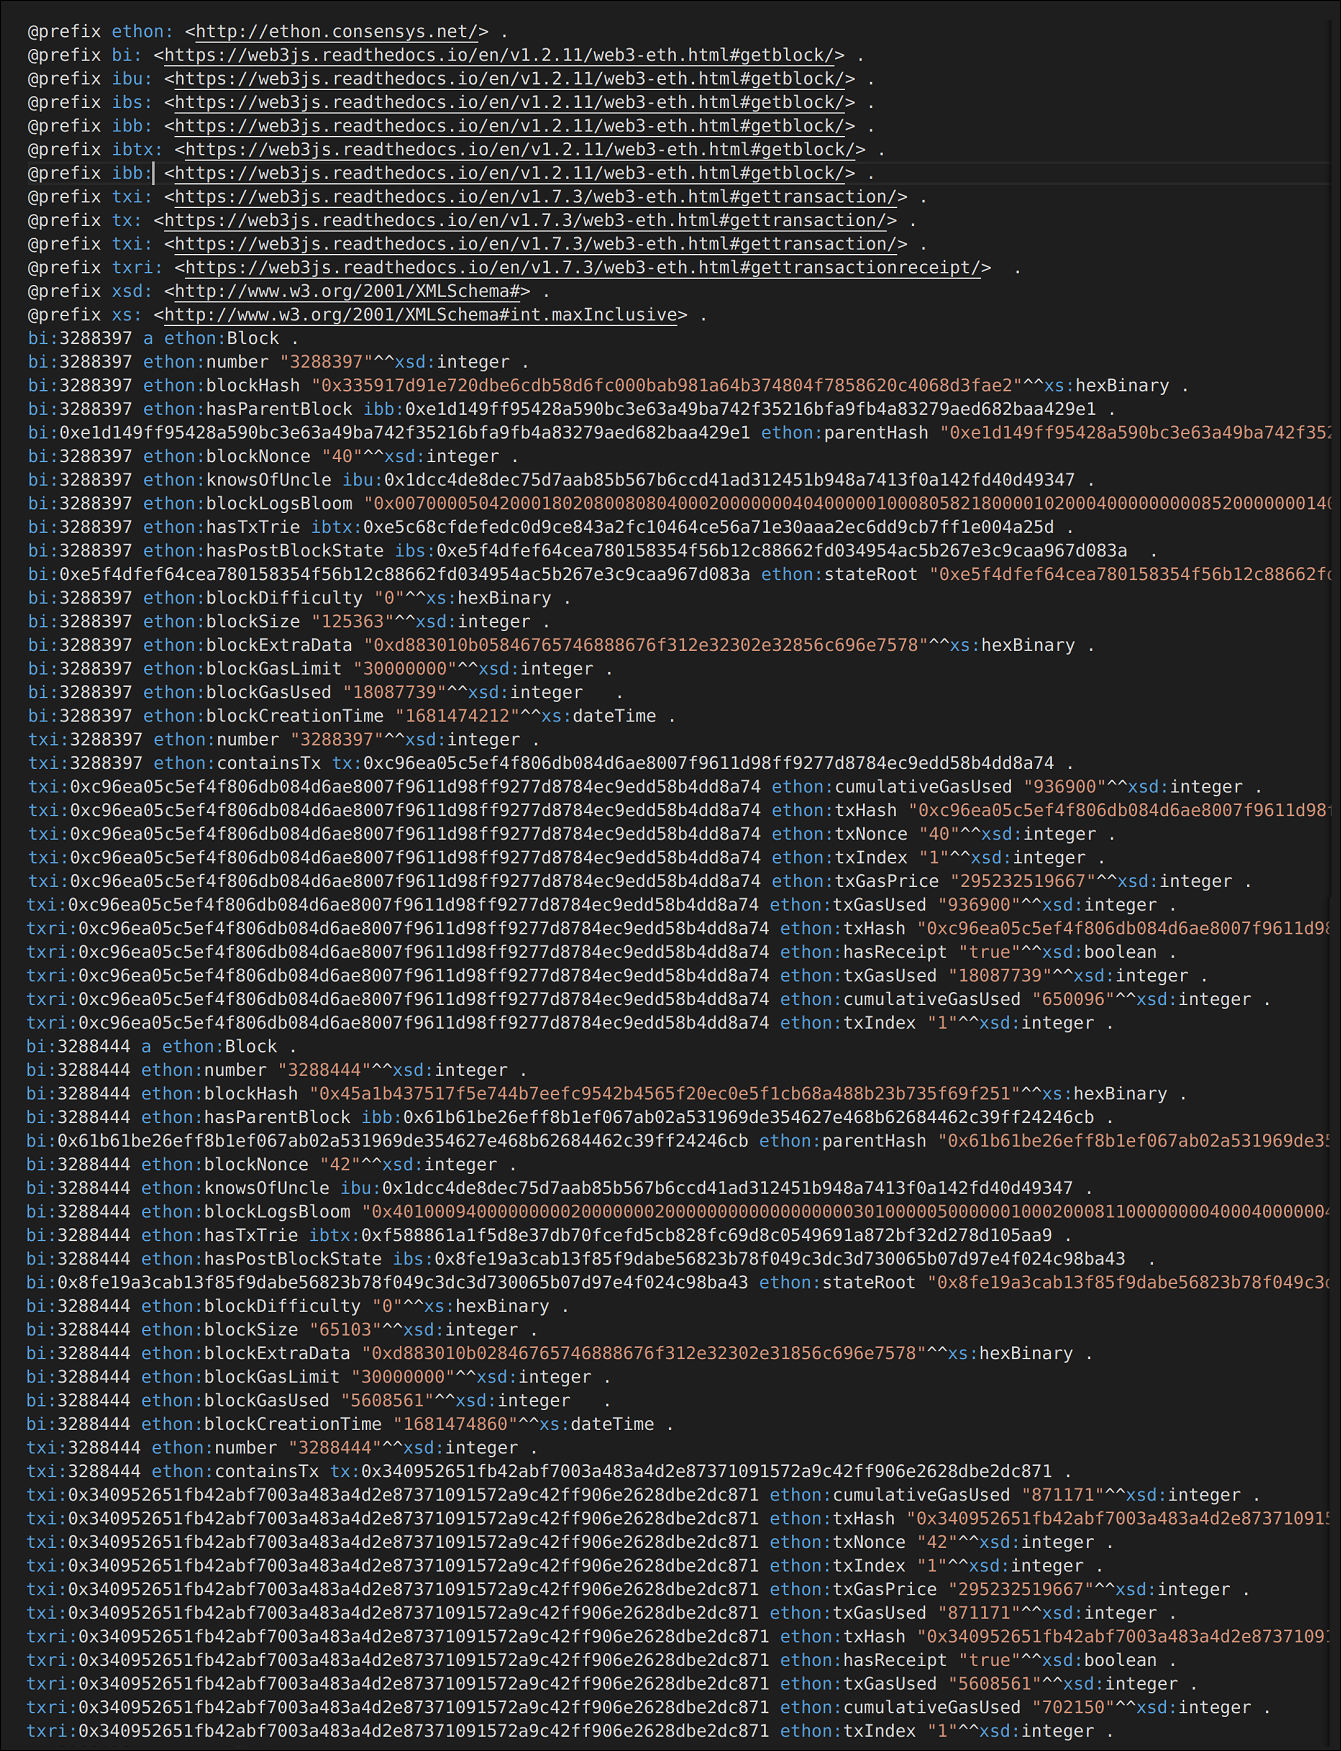
\includegraphics[width=1.95\textwidth]{images/chap03_triple_result.png}
		\end{minipage}
		
	\end{figure}
	
\end{center}
\bibliographystyle{apalike}
\bibliography{biblio}
%next line adds the Bibliography to the contents page
\addcontentsline{toc}{chapter}{Bibliography}
%uncomment next line to change bibliography name to references
%\renewcommand{\bibname}{References}
%\bibliography{refs.bib}        %use a bibtex bibliography file refs.bib
%\bibliographystyle{plain}  %use the plain bibliography style

\end{document}

